\documentclass{article}
\usepackage[margin=20mm]{geometry}
\usepackage[hidelinks]{hyperref} % Conflicted with new SV template
%\usepackage{lastpage}       % ``n of m'' page numbering
%\usepackage{lscape}         % Makes landscape easier
%\usepackage{verbatim}       % Verbatim blocks
\usepackage{listings}       % Source code listings
\usepackage{epsfig}         % Embed encapsulated postscript
\usepackage{array}          % Array environment (advanced tables)
\usepackage{hhline}         % Horizontal lines in tables
\usepackage{siunitx}        % Correct spacing of units
\usepackage{amsmath}        % American Mathematical Society
\usepackage{amssymb}        % Maths symbols
\usepackage{amsthm}         % Theorems & QED
%\usepackage{ifthen}         % Conditional processing in tex
\usepackage{parskip}
\usepackage{float}
\usepackage{amsmath} % for the \DeclareMathOperator macro
\allowdisplaybreaks % From amsmath: allows align to span pages
\usepackage{centernot}
\usepackage{mathtools} % for small matrices
\newcommand{\bmat}[1]{\begin{bmatrix}#1\end{bmatrix}}
\usepackage{cancel}
\usepackage{amsthm}
\theoremstyle{definition}
\newtheorem{theorem}{Theorem}
\newtheorem{lemma}[theorem]{Lemma}
\DeclareMathAlphabet{\mathbbb}{U}{bbold}{m}{n}  % for things like \mathbb{1} to work, courtesy of https://tex.stackexchange.com/a/601142
\usepackage{cmap} % allow ff / fi ligatures to be searchable
\usepackage{enumitem} % For custom enumerate
%\usepackage[hidelinks]{hyperref} % Conflicted with new SV template
\usepackage[nottoc]{tocbibind} % Adds References to TOC. Though recommended, note that this command can mess up certain things (e.g. fancyhf in fancyhdr, among other things mentioned at https://www.overleaf.com/learn/latex/Bibliography_management_with_bibtex#Adding_the_bibliography_in_the_table_of_contents)
\usepackage{cite} % compress long lists of citations like [1, 2, 3, 4] into [1--4]. Courtesy of https://tex.stackexchange.com/a/15114
\usepackage{graphicx}
\usepackage{graphbox}  % adds [align=c] option to includegraphics, courtesy of https://tex.stackexchange.com/a/350374
\usepackage{multirow}
\usepackage{xcolor}
\usepackage[T1]{fontenc} % what's this for? https://tex.stackexchange.com/questions/664/why-should-i-use-usepackaget1fontenc
\usepackage{lmodern} % fixes pixelation
\newcommand{\textgrey}[1]{\textcolor{gray}{#1}}
\DeclareMathOperator*{\argmin}{argmin}
\usepackage{mathrsfs}
% Boilerplate for appendix TOC courtesy of https://tex.stackexchange.com/a/419290
\usepackage{minitoc}
\renewcommand \thepart{}
\renewcommand \partname{}

\def\vt#1{\underline{\mathbf{#1}}}
\def\vts#1{\underline{\boldsymbol{#1}}}
\def\mt#1{\underline{\underline{\mathbf{#1}}}}
\def\mts#1{\underline{\underline{\boldsymbol{#1}}}}

% Courtesy of https://tex.stackexchange.com/a/106719
\usepackage{stmaryrd}
\SetSymbolFont{stmry}{bold}{U}{stmry}{m}{n}
                                     %%%

\graphicspath{ {imgs/}{components/imgs/} }

%\setcounter{section}{-1}

\usepackage{multicol}
\title{Image matting}
\author{Jacky~W.E.~Kung}
\date{15 January 2024}

\setlength{\columnsep}{0.5cm}
\begin{document}
% Boilerplate for appendix TOC courtesy of https://tex.stackexchange.com/a/419290
\doparttoc % Tell to minitoc to generate a toc for the parts
\faketableofcontents % Run a fake tableofcontents command for the partocs


\maketitle
\begin{abstract}
    Image matting is a well-understood problem, and there exists closed-form solutions. However, as the problem is fundamentally underdetermined, there is no single ``correct'' solution, and thus algorithms in literature have considerable flexibility in defining what a ``best'' solution is and how to obtain it. This work reimplements one sampling-based and one propagation-based classical matting algorithm, and discusses code optimisation strategies. A detailed mathematical treatment of the underlying concepts is consolidated and presented. Quantitative and qualitative comparisons with today's state of the art deep learning algorithm are presented. The mathematical notation adopted in this work is outlined in Appendix~\ref{appendix:notation}.
    \textbf{ ANY QUANTITATIVE RESULTS TO REPORT? DO THEY MATCH THE ORIGINAL?  potential robust matting skill issue.. }
\end{abstract}
\begin{multicols}{2}[]



%In paper: less equations, more comparisons. Potentially change parameters (e.g. window size: graph: hyperparameter sweepish).

\section{Introduction}
% \emph{The "Introduction" section should briefly describe the proposed technique/modification/application, but above all, it should motive the work. Why is this work worth doing and the paper worth reading?}
%https://people.csail.mit.edu/fredo/FredoGoodWriting.pdf
%• Motivation
    %- need or opportunity
%• Context
%• First overview of your contributions, focusing on big ideas and silver bullets
%• Consequences & benefits
%• Possibly summary of contributions (what ideas are new)
    %- can be useful when you only modified some parts of a bigger technique

%• Forget what you thought an overview was
%- I hate “In section we introduce blah, in section 2....)

The process of matting an image involves separating foreground objects from the background. Formally, the matting equation is defined at each pixel $k$ of the image $\mt I$ by $$\vt I_k = \alpha_{k} \vt F_{k}  + (1-\alpha_k) \vt B_k$$
where $\alpha_{k}\in[0,1]$, and $\mt F, \mt B$ are the unknown ``foreground'' and ``background'' images. Explicit definition of mathematical symbols are in Appendix~\ref{appendix:theorem-1-statement}.   The alpha mask is fractional to allow smooth handling of fine details such as hairs, and also for motion blurring \cite{bayesian-matting}. The image matting problem is then to estimate $\vts \alpha, \mt F, \mt B$ using $\mt I$ and additional information from a user. This can take the form of \emph{trimaps}, in which the user annotates pixel regions that are definitely foreground, definitely background, and ambiguous.  The traditional green/blue screen technique works, but we are interested in matting for general images that do not have a monochrome background.

To the best of my knowledge, only a \verb|C++| implementation \cite{web:robust-cpp-github} exists for Robust Matting \cite{robust-matting}, and it cannot be compiled in 2024 due to outdated dependencies.  This work reimplements both Robust Matting and Closed-form Matting \cite{closed-form-matting} in Python. While there exists a Python implementation for the latter \cite{web:closed-form-python-github}, reimplementation without referring to it was done to obtain a deeper understanding of its mathematical foundations, which are also necessary for understanding Robust Matting. Furthermore, this work presents an evaluation of various sampling strategies for Robust Matting, which was left out in the original paper. Finally, a brief performance comparison with today's state of the art deep neural network (DNN) algorithm is performed.




%“Although the problem is severely ill-posed, the strong correlations between nearby image pixels can be leveraged to alleviate the difficulties.” ([Wang and Cohen, 2007, p. 1](zotero://select/library/items/82ECWWKJ)) ([pdf](zotero://open-pdf/library/items/H4SBS9AI?page=1))

% Questions: What if we specify everything as ambiguous? Will sampling fail? Will propagation fail?

%“Although various successful examples have been shown for these approaches, their performance rapidly degrades when foreground and background patterns become complex. The intrinsic reason is that in many images the foreground and background regions contain significant textures and/or discontinuities;” ([Wang and Cohen, 2007, p. 1](zotero://select/library/items/82ECWWKJ)) ([pdf](zotero://open-pdf/library/items/H4SBS9AI?page=1))


\section{Related Work}
% \emph{The "Related work" section should review 2-4 relevant papers, compare and contrast the proposed work to what has been published before.}

Classical matting algorithms are split into two classes. \emph{Sampling-based} methods first estimate $\vt F_k$ and $\vt B_k$ by sampling known foreground and background pixels marked by a provided trimap, then solve for $\alpha_k$ \cite{dim-paper}. Bayesian Matting solves for the maximum a posteriori (MAP) estimate for $\vts \alpha,\mt F,\mt B$ simultaneously \cite{bayesian-matting}. Robust Matting computes a confidence measure for foreground-background sample pairs, and chooses those with the highest confidence as the samples. This work focuses on Robust Matting as it is newer and better performant than Bayesian Matting. \emph{Propagation-based} methods transfer information about known alphas from annotated foreground and background regions into the unknown ambiguous regions \cite{dim-paper}. Poisson Matting solves a Poisson equation using a desired alpha gradient field \cite{poisson-matting}. Closed-form Matting produces $\vts \alpha$ by solving of a system of sparse linear equations, and is a seminal piece of work influencing many later algorithms. Again, this work focuses on Closed-form matting as it is newer and better than Poisson matting. Newer matting algorithms exist for both classes \cite{closed-form-survey}, but are outside the scope of this work.  %\cite{closed-form-matting} is the newest and most superior of these four techniques, and

State of the art approaches today involve DNNs. The best performing algorithm on the \emph{Composition-1K} dataset at time of writing is \emph{AEMatter}, according to \emph{PapersWithCode}. As its authors explain, DNNs supersede classical algorithms with their ability to capture and represent complicated high-level context (e.g.\ common patterns in hairs), significantly improving the quality of mattes produced \cite{sota-composition-1k}. We compare the chosen classical algorithms with AEMatter in the evaluation section (\S\ref{evaluation}).

% The proposed plan of this project is to:
% \begin{enumerate}[label=\arabic*.]
%     \item Re-implement, adapting code wherever possible, \textbf{Closed-Form Matting} (propagation-based) and \textbf{Optimised Colour Sampling} (sampling-based). If time permits (pending discussion of final project scope with supervisor), the other two mentioned classical methods may be implemented too. The aim is to achieve deep understanding of these classical methods.
%     \item Compare the results between these two classes of methods:
%     \begin{itemize}
%         \item (Qualitative) The four papers provided in the synopsis \cite{bayesian-matting, robust-matting, poisson-matting, closed-form-matting} rely mainly on qualitative evaluation on a small number of ``problematic'' images. These would be sourced from more recent literature.
%         \item (Quantitative) Some of the four papers use metrics such as \emph{mean squared error} or \emph{mean absolute error} (MAE) between ground-truth and predicted mattes $\alpha$. MAE is also known as \emph{alpha loss} in deep learning literature \cite{dnn-survey}.

%         Deep learning methods use a much wider variety of metrics, including \emph{composition loss}, \emph{Laplacian loss} and \emph{cross entropy loss} \cite{dnn-survey}. An attempt would be made to evaluate the re-implemented classical methods using some of these metrics.
%     \end{itemize}
%     \item If the scope of the project will not become too big (pending discussion with supervisor), and if time and resources permit, use existing code for a state-of-the-art deep learning model, and compare its performance against the classical methods. An attempt would be made to corroborating the explanations of of Liu et al.\ \cite{sota-composition-1k} regarding the superiority of neural networks over classical methods.
% \end{enumerate}

%SAMPLING
%Bayesian: few test images
%Optimised colour: MSE with 8 test images
%
%PROPAGATION
%Poisson: few test images
%Closed-form: discussion of few test images (known to be hard for the time). Quantitative numbers: summed absolute error [alpha loss] Application to classical methods?

%Mostly qualitative. Quantitative metrics (also from Image and Video Quality Assessment lecture coming up)
%
%Deep learning: many kinds of losses.





%https://people.csail.mit.edu/fredo/FredoGoodWriting.pdf
%• Focus on how they inform, motivate and differ from your work
%• Can provide a self-contained introduction to the field
%• Sometime also add a tutorial on required background that is uncommon in the field
%• Be generous. Don’t piss off people.




%
%[Deep survey] Performance benchmarking... losses.
%[Rethinking Context aggregation] Why NNs are used; and currently one of the SOTA (for dataset from DIM paper). Deep learning-based methods [52, 31] use an encoder to extract context features from the input and then estimate the alpha matte through a decoder, as shown in Figure 1(a). Due to the powerful representation ability of the learned context features, these methods significantly outperform traditional sampling-based and propagation-based methods.

%Closed form: code in objective-C is provided. Might want to re-implement in a more modern language? See if it already exists. Solves for alpha, then F and B.
%Optimisation: alpha, then F and B
%Estimate F,B then alpha, then F,B. Iterative.



%[DIM] create a large-scale image matting dataset including 49300 training images and 1000 testing images.  [Composition-1K] Points out assumptions where classical methods fall (relying on colour and spatial position of pixels as the distinguishing feature, thus sensitive to FG/BG distributions overlapping (common for natural images))

% \textbf{Do classical method research stop at Optimised Colour Sampling? Can my related work be limited to these 4/2/(2+1ML) papers?}


% \begin{itemize}
%     \item Bayesian 2001: a primitive sampling method, but non-interactive. Uses trimap.
%     \item Poisson 2004: an improved propagation method, interactive (seminal propagation method paper?). Uses trimap. Fits oriented Gaussians to foreground and background images to learn then, then picks best aFB given the learned distribution.
%     %“First, when the foreground and background colors are very similar, the matting equation becomes ill-conditioned. In this case, the underlying structure of the matte can not be easily distinguished from noise, background or foreground.” ([Sun et al., 2004, p. 320](zotero://select/library/items/QZ8DCSDY)) ([pdf](zotero://open-pdf/library/items/PB4T6VTX?page=6))
%     %“where a mixture of oriented Gaussians is used to learn the local distribution and then , F , and B are estimated as the most probable ones given that distribution. Such methods work well when the color distributions of the foreground and the background do not overlap, and the unknown region in the trimap is small.” ([Levin et al., 2008, p. 229](zotero://select/library/items/TDAQSBJL)) ([pdf](zotero://open-pdf/library/items/ISLA8TYD?page=2))
% \end{itemize}
% \begin{itemize}
%     \item Closed-Form Matting 2006: a propagation method. Doesn't \emph{necessarily} use trimaps. Argues trimaps are a limitation, and user interaction to refine trimap shouldn't be needed. Uses just a SPARSE set of scribbles from user since reliable estimates for F and B images are not required for this method. \textbf{CODE AVAILABLE. But it's in Objective-C...}

%     Can be seen as a smoothness refinement technique: \emph{``Smoothness refinement method is a straightforward idea that first utilizes sampling-based strategy to estimate the alpha matte and then refines the alpha matte using affinity-based strategy.''}
%     %“This is typically done by iterative nonlinear optimization, alternating the estimation of F and B with that of alpha. In practice, this means that for good results, the unknown regions in the trimap must be as small as possible. As a consequence, trimap-based approaches typically experience difficulty handling images with a significant portion of mixed pixels or when the foreground object has many holes [19].” ([Levin et al., 2008, p. 228](zotero://select/library/items/TDAQSBJL)) ([pdf](zotero://open-pdf/library/items/ISLA8TYD?page=1))
%     \item Optimised Colour Sampling (i.e.\ Robust Matting) 2007: the latest (of the four) sampling method.  Addresses lack of systematic comparison. Builds upon closed-form matting.
% \end{itemize}


%The methods may have different kinds of biases (different types of images). Sharp edges, noise, etc. METRICS.


\section{Method}
% \emph{The "Method" section should clearly explain the technique, focusing on why certain decisions were taken, rather than just reporting the work that has been done. It should explain the method with the help of equations and illustrations, as appropriate.}
%https://people.csail.mit.edu/fredo/FredoGoodWriting.pdf

%For initial iteration, crop a small part of the image. Only for final testing use full images!!

This Before implementing the two algorithms, I sought a deep understanding of their mathematical foundations. I will present some of the useful insights here, along with how they affect the code implementation.

\subsection{Closed-form Matting}\label{s3-closed-form-matting}
The Python implementation was written by consulting the MATLAB implementation provided by the authors, as there are many crucial details expressed not in the original paper but only through their code. I present the important ones here.

For coloured images with height $H$ and width $W$, %Closed-form Matting assumes the \emph{colour line model}, which states that within any local window of an image, all foreground pixels can be expressed as a linear combination of two colours, and likewise for background pixels. This allows us to predict the alpha value of a pixel $\alpha_{k}$ linearly from the pixel value $\vt I_{k}$ as $\alpha_k = \vt a_k^T \vt I_k + b_k$ for some vector $\vt a_k^T$ and scalar $b_k$.
Theorem 1 \cite{closed-form-matting} defines the loss of a predicted alpha image $\vts \alpha$ as $ J(\vts \alpha) = \vts \alpha^T \mt L\, \vts \alpha$ where $\vts \alpha$ is a length-$HW$ vector, and $\mt L$ is a $HW\times HW$ sparse \emph{matting Laplacian} matrix with entries defined below. A full derivation, not present in literature to be best of my knowledge, is presented in Appendix~\ref{appendix:theorem-1}.
% \begin{center}
%     \resizebox{0.65\columnwidth}{!}{%
%     $\begin{aligned}[t]
%         J(\vts \alpha) &= \sum_{k\in K} \overbracket{\min_{\mt a_k,\vt b_k}  \left(\sum_{m=0}^{M^2-1} \left(\alpha_{n_m} - \vt a_k^T \vt I_{n_m} - b_k\right)^2 + \epsilon \vt a_k^T \vt a_k \right)}^{(**)} \\
%         &= \vts \alpha^T \mt L \, \vts \alpha
%     \end{aligned}$
%     }
%     \end{center}

\resizebox{\columnwidth}{!}{%
$\displaystyle L_{i,j} = \sum_{\substack{k\in K:\\i\in w_{(k)}\\\wedge j\in w_{(k)}}} \left( \delta_{ij} - \underbracket{\frac1{M^2}\left(1 + \left(\vt{I}_i - \vts \mu_{(k)}\right)^T \left(\mts \Sigma_{(k)} + \frac\epsilon{M^2} \mt{I}_{3\times 3}\right)^{-1} \left(\vt{I}_j - \vts \mu_{(k)}\right) \right)}_{(*)} \right). $
}

Even for low resolution images of size $600 \times 400$, $\mt L$ is a $240\text{k} \times 240\text{k}$ matrix, which contains $\SI{5.76e10}{}$ cells. Thankfully, sparse matrix libraries such as \verb|scipy.sparse| exist to alleviate space usage, and runtime can be significantly sped up by skipping over unnecessary sums.

\paragraph{Skipping $k$s when computing $\mt L$.} To see this, the closed-form solution $\hat{\vts\alpha}$ is found via Lagrangian optimisation as
$$\hat{\vts \alpha} = \argmin_{\vts\alpha} \left( J(\vts\alpha) + \lambda \left(\vts\alpha - \vt b_S\right)^T\mt D_S \left(\vts\alpha - \vt b_S\right) \right)$$
where $\mt D_S$ is a $HW\times HW$ diagonal matrix whose element is 1 if that pixel is known (to be foreground or background) and 0 otherwise, $\vt b_S$ is a length-$HW$ vector containing the known alpha values (1 for foreground, 0 for background and unknown), and $\lambda=100$ is a large Lagrangian multiplier to enforce the known alpha values. $J(\vts\alpha)$ thus predominantly only influences the unknown alpha values in $\hat{\vts\alpha}$. When computing $\mt L$ as part of $J(\vts\alpha)$, we may thus skip summing over centres $k$ where all pixels have known mattes, as such computation has imperceptible effect on the final $\hat{\vts \alpha}$.

\textbf{Computation of $\mt L$.} A triple for-loop iterating over all $i,j$ and then considering applicable centres $k\in K$ performs many repeated computations. The code instead iterates over all window centres $k\in K$, and computes the summand $(*)$ for all $M^4$ possible pixel pairs in the window, then adds them to the corresponding $M^4$ elements of a $HW\times HW$ sparse matrix $\mt W$ as illustrated by Figure~\ref{fig:index-displacement}. $\mt W$ is defined as
\resizebox{\columnwidth}{!}{%
$\displaystyle W_{i,j} = \sum_{\substack{k\in K:\\i\in w_{(k)}\\\wedge j\in w_{(k)}}} \frac1{M^2}\left(1 + \left(\vt{I}_i - \vts \mu_{(k)}\right)^T \left(\mts \Sigma_{(k)} + \frac\epsilon{M^2} \mt{I}_{3\times 3}\right)^{-1} \left(\vt{I}_j - \vts \mu_{(k)}\right) \right). $
}
% producing a $M^2\times M^2$ dense matrix $\mt W^{(k)}$ defined as

% \resizebox{\columnwid$\displaystyle W_{i,j} = \sum_{\substack{k\in K:\\i\in w_{(k)}\\\wedge j\in w_{(k)}}} \frac1{M^2}\left(1 + \left(\vt{I}_i - \vts \mu_{(k)}\right)^T \left(\mts \Sigma_{(k)} + \frac\epsilon{M^2} \mt{I}_{3\times 3}\right)^{-1} \left(\vt{I}_j - \vts \mu_{(k)}\right) \right). $_{x,y} = \frac1{M^2}\left(1 + \left(\vt{I}_{n_x} - \vts \mu_{(k)}\right)^T \left(\mts \Sigma_{(k)} + \frac\epsilon{M^2} \mt{I}_{3\times 3}\right)^{-1} \left(\vt{I}_{n_y} - \vts \mu_{(k)}\right) \right)$
% }

% for $x,y\in\{0,\dots, M^2-1\}$ and window $w_{(k)} = \{n_0,\dots,n_{W^2-1}\}$ and $n_0,\dots,n_{W^2-1}\in \{0,\dots,HW-1\}$.

% . Its values

\begin{figure}[H]
    \centering
    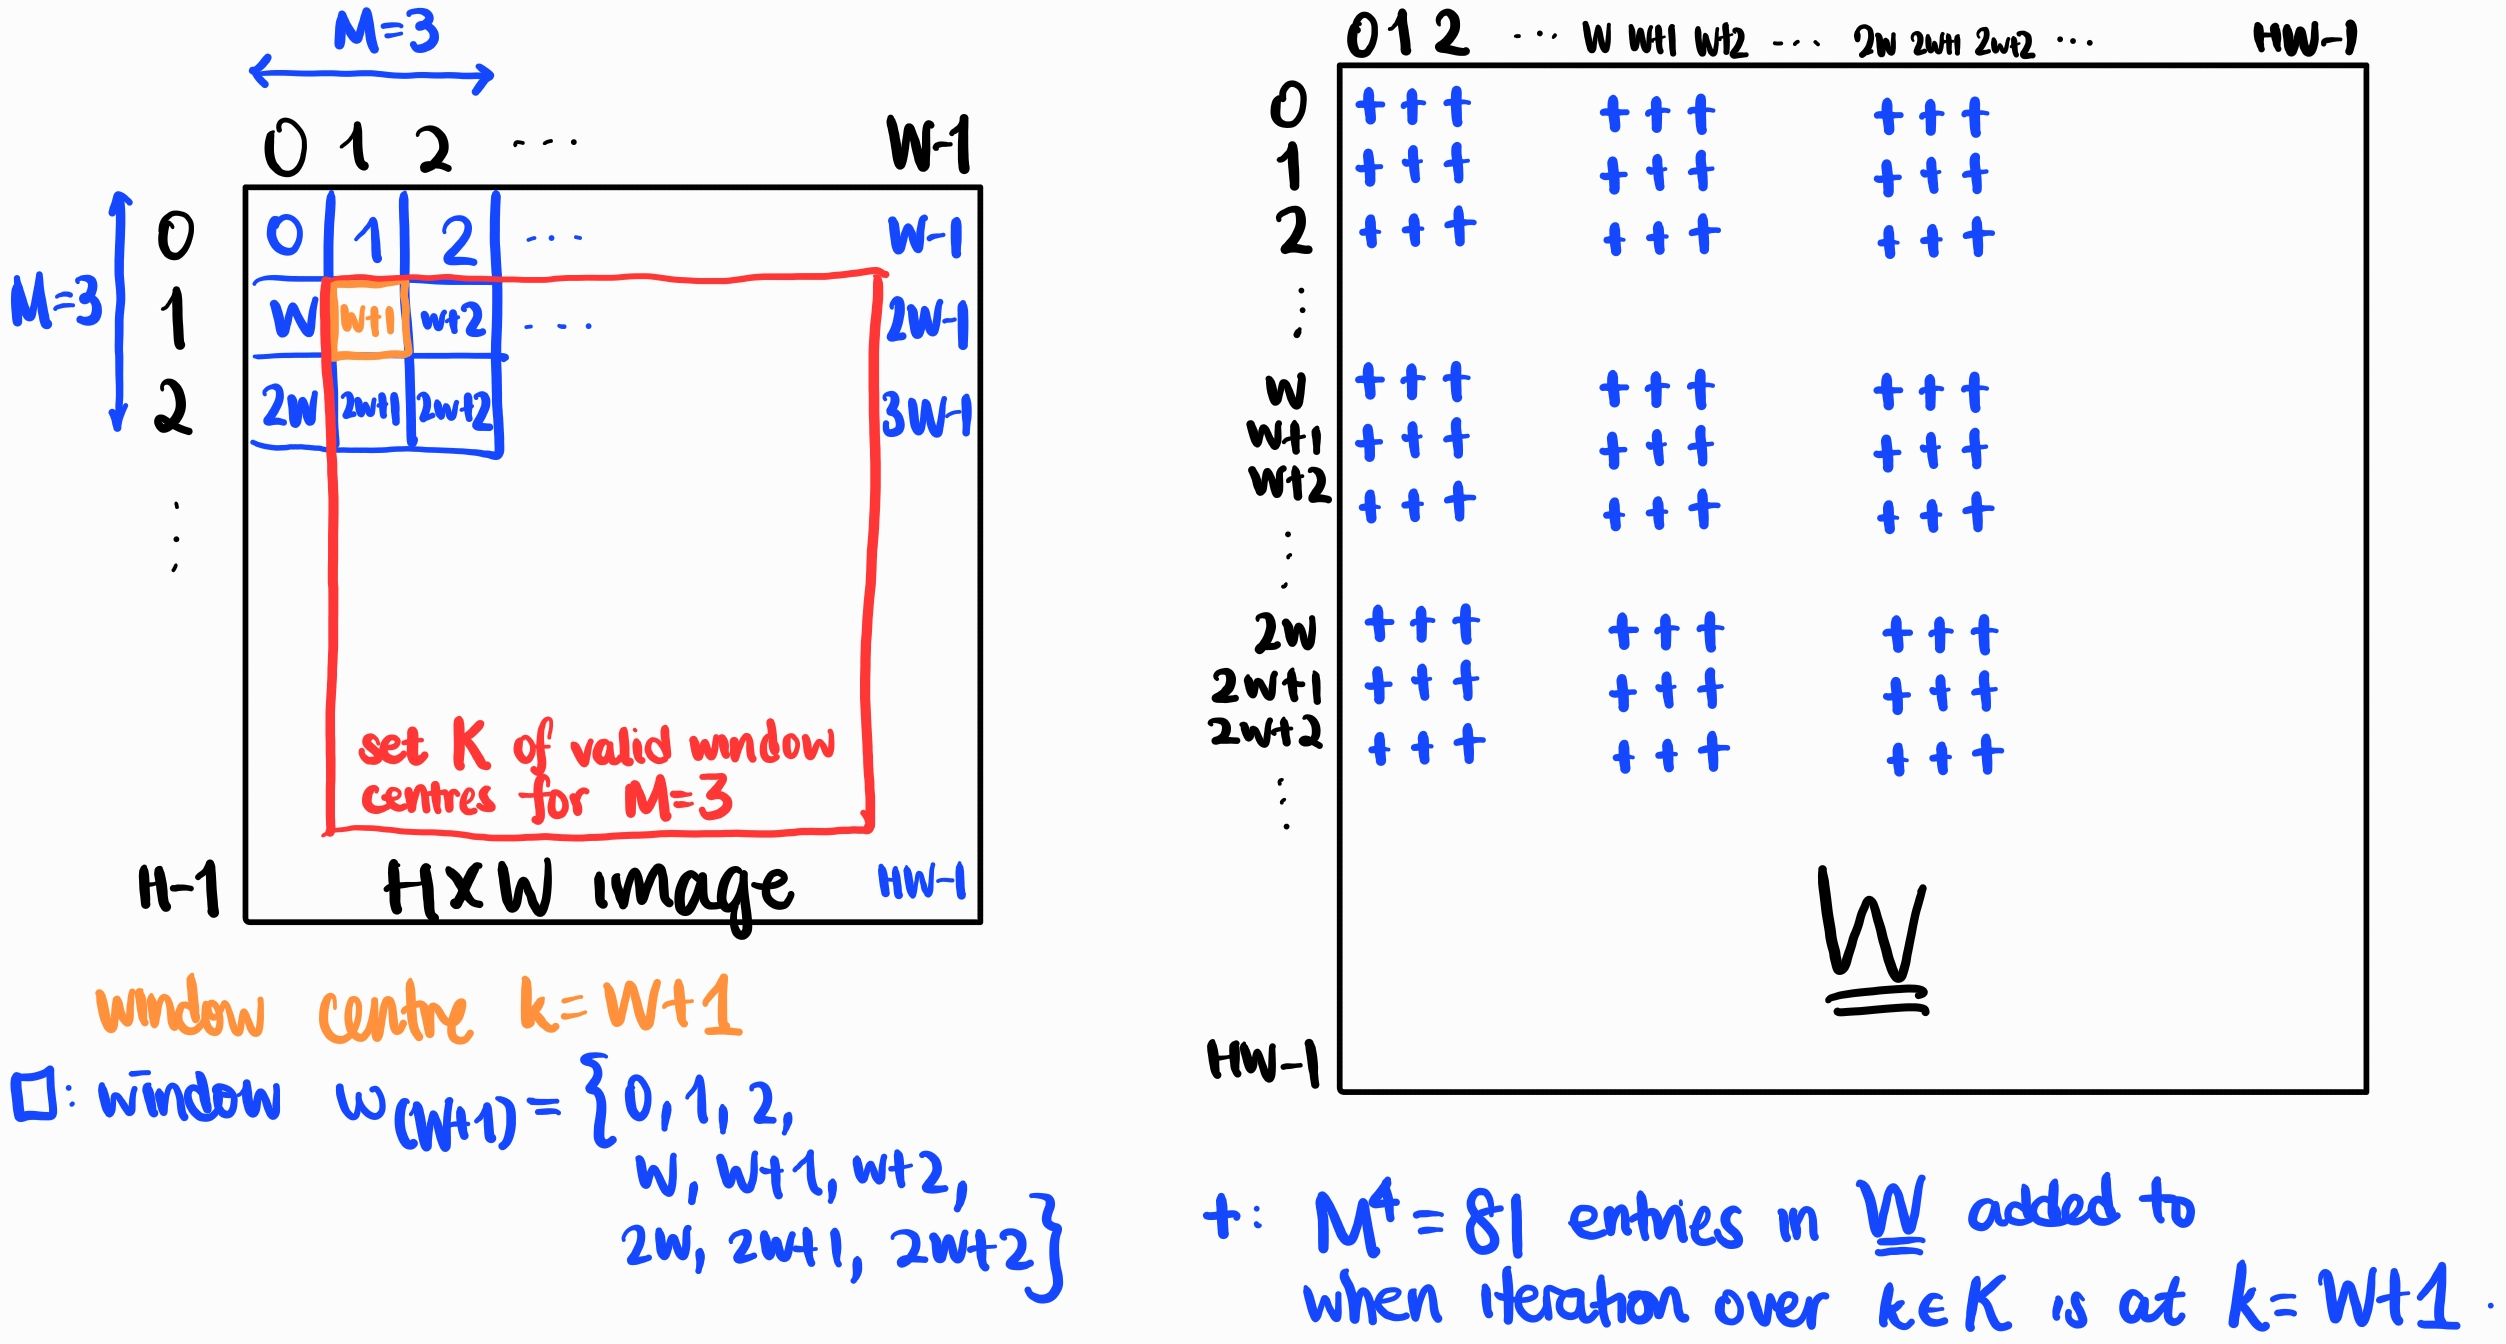
\includegraphics[width=\linewidth]{index-displacement}
    \caption{Left: Computation of $\mt L$ involves iterating over all possible window centres $k\in K$ (within the red box). Right: Values in $\mt W$ incremented during iteration $k=W+1$.}
    \label{fig:index-displacement}
\end{figure}
The $\delta_{ij}$ terms are handled by constructing a $HW\times HW$ diagonal matrix $\mt D$ whose entries are $D_{i,i} = \sum_{j=0}^{HW-1} W_{i,j}$, and $\mt L$ is finally given by $\mt L = \mt D - \mt W$. Proof of this method's correctness is provided in Appendix~\ref{appendix:w-sum-zero-proof}.

\paragraph{Optimisation overview}
The Lagrangian optimisation has a closed form solution
$$(\mt L + \lambda \mt D_S) \hat{\vts \alpha} = \lambda \mt D_S \vt b_S$$
which is computed via Cholesky decomposition with the \verb|sksparse.cholmod| library.

\paragraph{Coarse-to-fine computation of $\hat{\vts\alpha}$.} Computation of the full-size Laplacian may still take tens of seconds for large images. For efficiency, the implementation constructs a four-layer Gaussian pyramid. Computation of Laplacians and Lagrangian optimisation (to obtain downsampled $\hat{\vts\alpha}$) are performed only for the coarser two layers. Each time we move to the next finer layer, alpha values within $0.02$ of $0$ or $1$ are clipped to $0$ and $1$ respectively. The coarser $\hat{\vts\alpha}$ is used to compute the $\vt a_k^T, b_k$ terms in the colour line model equation $\alpha_k = \vt a_k^T \vt I_k + b_k$. These terms are then upsampled via linear interpolation, and the right-hand side of the same equation evaluated to obtain a finer $\hat{\vts\alpha}$. We defer details to the original paper, which showed that this procedure is efficient and produces a final $\hat{\vts\alpha}$ that is very similar to solving the full-size Laplacian directly \cite[\S4]{closed-form-matting}.
% constrain a pixel iff all pixels in its window are also constrained. For these centres, no need to enforce linear colour model,
%     # so we omit summing them. Remember the alphaT L alpha term is there to enforce the smoothness/linear colour models.
%     # I believe for these centres, the linear model is trivially satisfied and so no loss.





\subsection{Robust Matting}
The Python impelmentation was written with minimal reference (only referring to \cite{web:robust-cpp-github} for debugging). Robust Matting proceeds in two phases: sampling and optimisation.

\paragraph{Sampling overview.} Using a provided trimap, we binary-dilate the unknown regions using a simple $3\times 3$ ones kernel. Intersecting this with the foreground and background regions produces the foreground and background boundaries respectively. For each unknown pixel with pixel value $\vt I_k$, 20 foreground boundary and 20 background boundary pixels $\{\vt F_i\}_{i=0}^{19}, \{\vt B_j\}_{j=0}^{19}$ are sampled. For each of the 400 possible foreground-background sample pairs $(\vt F_i, \vt B_j)$, an alpha estimate $\alpha_{i,j} = \frac{\left(\vt F_i - \vt B_j\right)^T\left(\vt I_k - \vt B_j\right)}{\left(\vt F_i - \vt B_j\right)^T\left(\vt F_i - \vt B_j\right)}$ is computed using the projection of $\vt I_k$ onto the line through $\vt F_i$ and $\vt B_j$, and a confidence metric $f(\vt F_i, \vt B_j; \vt I_k)$ assigned. The top three highest confidence values and alphas are retained and averaged to form the initial confidence and alpha estimates $\hat f_k$ and $\hat{\alpha}_k$ respectively.

\paragraph{Computation of confidences.}
The mathematical form of $f(\vt F_i, \vt B_j; \vt I_k)$ presented here is equivalent to the one in original paper, but this form allows for common-subexpression elimination optimisations in my implementation.

\resizebox{\columnwidth}{!}{%
$\begin{aligned}[t]
    \mt A_{(i,j)} &\triangleq \frac{\mt I_{3\times 3} -  \frac{\left(\vt F_i - \vt B_j\right)\left(\vt F_i - \vt B_j\right)^T}{\left(\vt F_i - \vt B_j\right)^T\left(\vt F_i - \vt B_j\right)}}{\left(\vt F_i - \vt B_j\right)^T\left(\vt F_i - \vt B_j\right)} \\
    f(\vt F_i, \vt B_j; \vt I_k) &= \exp\left(\frac{-1}{\sigma^2} \left(
    \left(\vt I_k - \vt B_j \right)^T \mt A_{(i,j)}\left(\vt I_k - \vt B_j \right) \cdot \exp\left(  -\frac{\left\| \vt F_i - \vt I_k \right\|^2}{\min_i \left\| \vt F_i - \vt I_k \right\|^2} - \frac{\left\| \vt B_j - \vt I_k \right\|^2}{\min_j \left\| \vt B_j - \vt I_k \right\|^2} \right)
\right)\right)
\end{aligned}$
}

Together with appropriate use of 3D \verb|numpy| arrays, this reduces the runtime complexity of the sampling stage from quadratic-like to linear-like with respect to the total number of unknown pixels (observed via local testing). For a test $800\times 500$ image, the sampling runtime was reduced from $\approx\SI{2.5}{\minute}$ to $\approx\SI{30}{\second}$, which is a significant speedup. Proof of correctness is provided in Appendix~\ref{appendix:robust-confidence}.



\paragraph{Sampling strategies.}
The original paper suggests spreading out the foreground and background boundary samples, but leaves concrete details out. In this work, we implement six different sampling schemes. \verb|global_random| samples randomly from all boundary pixels; \verb|local_random| samples randomly from nearby boundary pixels; \verb|nearest| samples the nearest boundary pixels; \verb|global_spread| evenly spreads out the samples throughout all boundary pixels; \verb|local_spread| evenly spreads out samples throughout nearby boundary pixels. \verb|global_random_same| is similar to \verb|global_random| but all unknown pixels use the same samples. These are illustrated in Figure~\ref{fig:sampling}. We suspect that \verb|local_spread| would perform best as the samples are both localised and spread out, which retains relevance of samples to the unknown pixel while increasing the probability of finding a good pair. Technically, a brute force search between all possible pairs using the full foreground and background boundaries would find the best possible pair given the image and trimap, but since it is computationally too expensive to perform, sampling is necessary.
\begin{figure}[H]
    \centering
    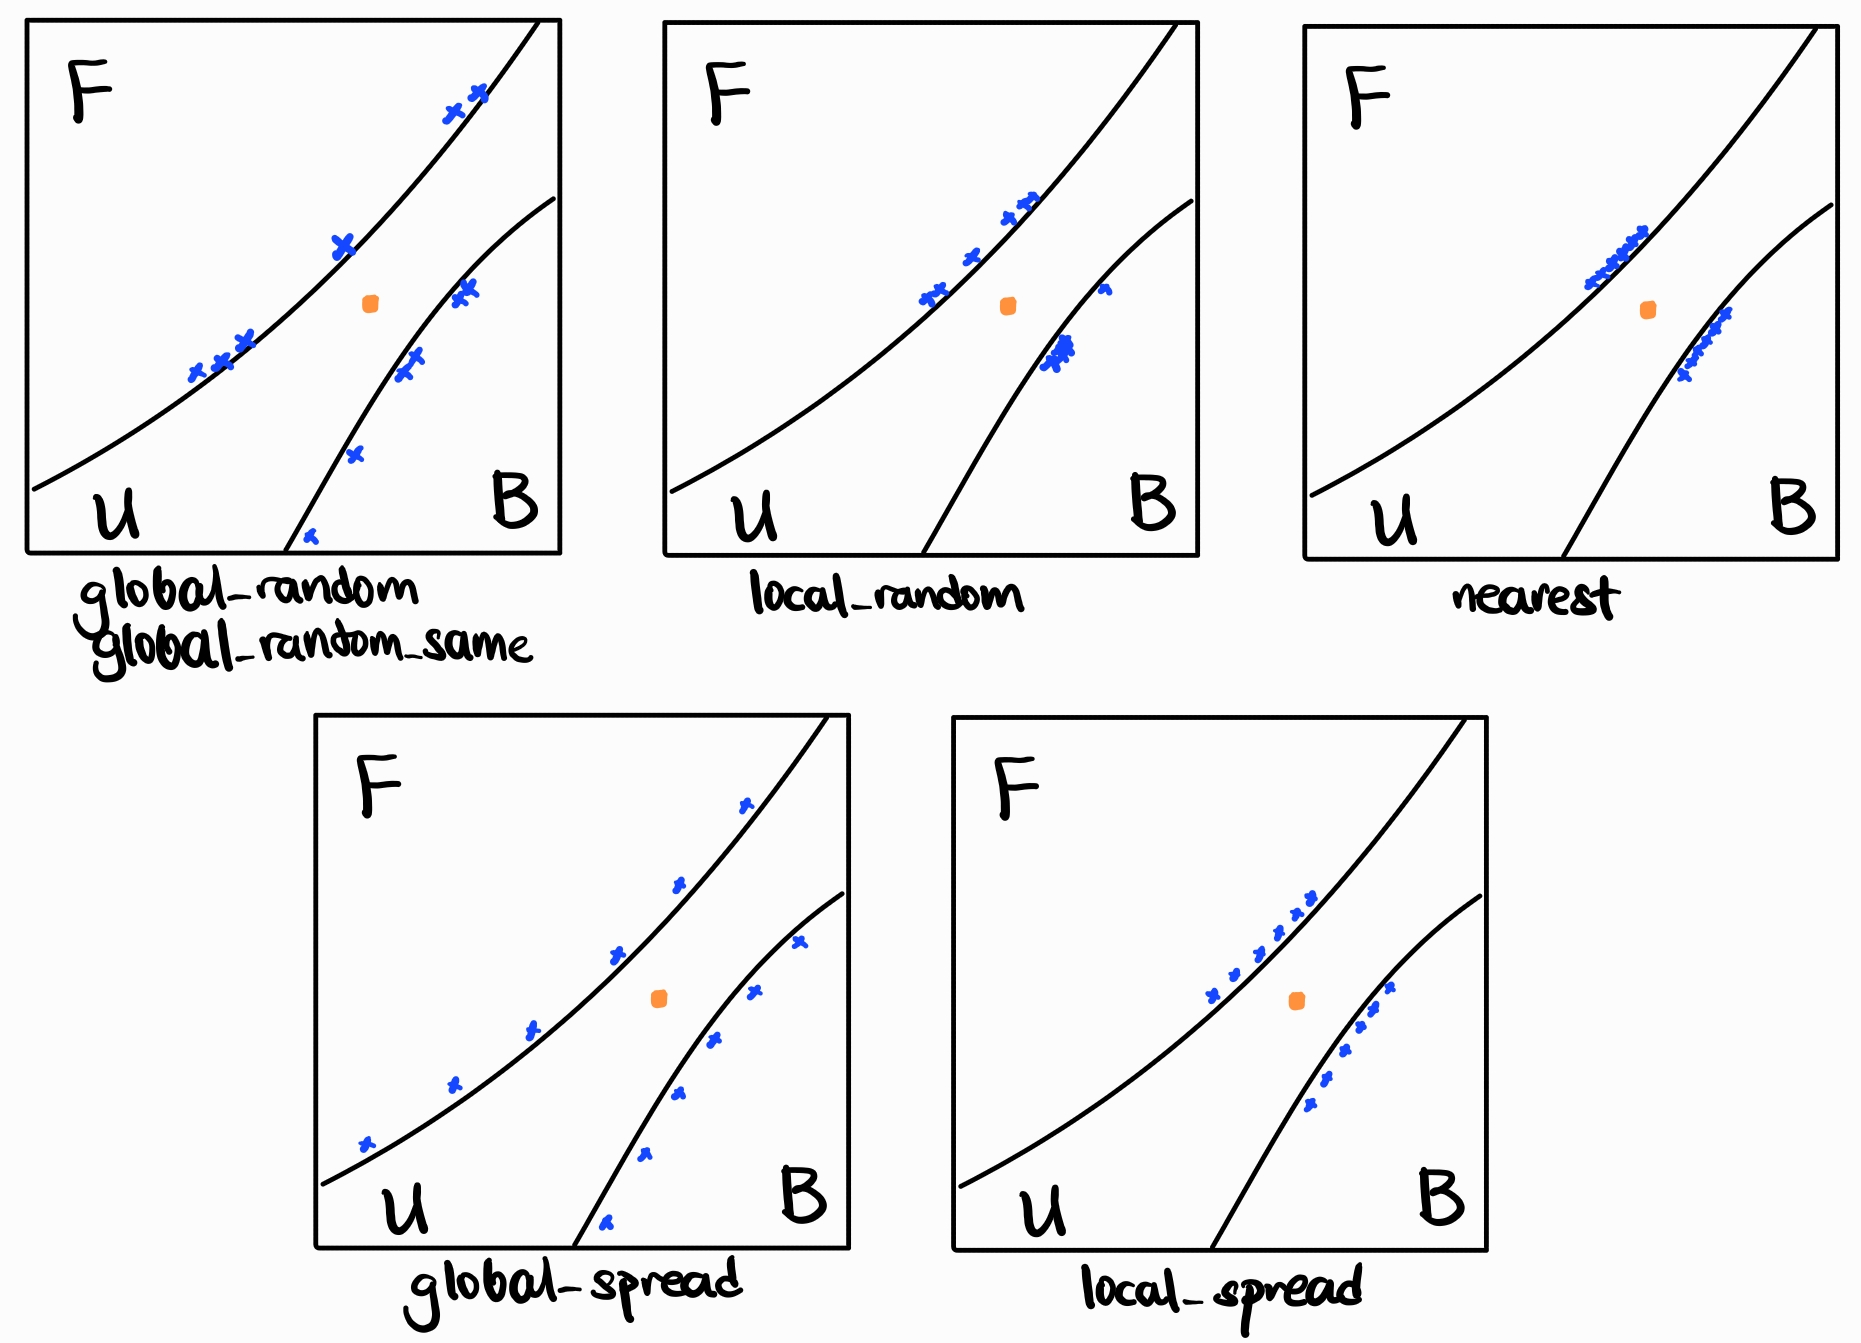
\includegraphics[width=0.7\linewidth]{sampling}
    \caption{The six implemented Robust Matting sampling strategies. $F,B,U$ represent foreground, background and unknown regions. The unknown pixel for which sampling is done is in orange, and the samples are in blue.}
    \label{fig:sampling}
\end{figure}

\paragraph{Optimisation overview.} Let $\#K$ and $\#U$ be the number of pixels in the original image with known and unknown alpha values respectively. We define length-$\#U$ vectors $\vt W^{(F)}, \vt W^{(B)}$ whose elements are defined as
\begin{align*}
    W^{(F)}_k &= \gamma\cdot\left(\hat f_k \hat{\alpha}_k + (1-\hat f_k) \mathbbb{1}_{\hat{\alpha}_k > 0.5} \right)\\
    W^{(B)}_k &= \gamma\cdot\left(\hat f_k \left(1-\hat{\alpha}_k\right) + (1-\hat f_k) \mathbbb{1}_{\hat{\alpha}_k \leq 0.5} \right)
\end{align*}
where $\mathbbb1_\text{predicate}$ is 1 if the predicate is true and 0 otherwise. The $(HW+2)\times(HW+2)$ matting Laplacian is then constructed as
$$\mt L = \left[\begin{smallmatrix}
    \times & \times & \times & \left(\vt W^{(F)}\right)^T \\
    \times & \times & \times & \left(\vt W^{(B)}\right)^T \\
    \times & \times & \mt L^{(1)} & \mt R \\
    \vt W^{(F)} & \vt W^{(B)} & \mt R^T & \mt L^{(u)}
\end{smallmatrix}\right]$$
where the first two rows and columns represent the virtual nodes $\Omega_F,\Omega_B$ mentioned in the paper \cite[\S4.3]{robust-matting}, $\mt L^{(1)}$ is a $\#K \times \#K$ matrix, and irrelevant submatrices are crossed out. The submatrix $\left[\begin{smallmatrix}\mt L^{(1)} & \mt R \\ \mt R^T & \mt L^{(u)}\end{smallmatrix}\right]$ is exactly the Laplacian we constructed for Closed-form Matting, except we reorder rows and columns such that when we index each axis from $0,\dots,HW-1$, all the known pixels come first, followed by all the unknown pixels. Importantly, this Laplacian has all the properties discussed in Section \ref{s3-closed-form-matting}. In particular each diagonal element is the negative sum of the rest of the row (since $\mt L = \mt D - \mt W$), therefore we must subtract from $L^{(u)}_{i,i}$ the sum of $W^{(F)}_i$ and $W^{(B)}_j$, which is $\gamma=0.1$. The unknown alpha values $\vt A_u$ in $\hat{\vts \alpha}$ is then found via Conjugate Gradient:
$$\mt L_u \vt A_u = -\mt R^T \vt A_k$$
where $\vt A_k$ is a length $(2+\# K)$ vector containing 1s for foreground pixels and 0s for background pixels.

\subsection{AEMatter}
The Python code provided by the authors is used as is, with minor modifications to enable usage on \emph{Google Colab}.

\section{Evaluation}\label{evaluation}
\emph{The "Evaluation" section should compare the method to the state-of-the-art, provide an evidence for improvement (or lack of it). The reported results should also show the limitations of the technique.}
%https://people.csail.mit.edu/fredo/FredoGoodWriting.pdf
%• Your results should support your claims
%• Be critical
%• again, get external feedback

%Evaluate on Multiple images
%http://alphamatting.com/datasets.php
% For closed form, manipulate trimaps to get scribbles? Trimaps most difficult to do.

%Evaluate for 3 different methods
%Crop a small area and focus on it. Close ups.

%PSNR equivalent to MSE. (supervisor)
%MSE within unknown area

Jesus christ this table is hard to insert
% \begin{table}[H]
%     \centering
%     \resizebox{\columnwidth}{!}{%
%     \begin{tabular}{@{}llccc@{}}
%     \toprule
%     \multicolumn{2}{c}{\textbf{Algorithm}} & \textbf{SAE} & \textbf{MSE} & \textbf{Time Taken [s]} \\ \midrule
%     \multirow{14}{*}{Robust} & \texttt{global_spread} & 10325k & 2665 & 56.5 \\
%      & \texttt{global_random_same} & 10038k & 2615 & 38.5 \\
%      & \texttt{global_random} & 10159k & 2564 & 41.3 \\
%      & \texttt{local_spread (nearest 1000)} & 9112k & 2209 & 56.6 \\
%      & \texttt{local_random (nearest 1000)} & 9017k & 2157 & 63.1 \\
%      & \texttt{local_spread (nearest 500)} & 8275k & 1967 & 56.6 \\
%      & \texttt{local_random (nearest 500)} & 8233k & 1935 & 61.7 \\
%      & \texttt{local_spread (nearest 200)} & 7019k & 1615 & 56.4 \\
%      & \texttt{local_random (nearest 200)} & 6966k & 1588 & 61.1 \\
%      & \texttt{local_spread (nearest 100)} & 6094k & 1360 & 56.2 \\
%      & \texttt{local_random (nearest 100)} & 6065k & 1345 & 60.9 \\
%      & \texttt{local_random (nearest 50)} & 5390k & 1201 & 60.7 \\
%      & \texttt{local_spread (nearest 50)} & 5188k & 1169 & 56.1 \\
%      & \texttt{nearest} & 4768k & 1113 & 55.9 \\
%     \multicolumn{2}{l}{Closed-form} & 1949k & 450.2 & 3.47 \\
%     \multicolumn{2}{l}{AEMatter} & \textbf{611k} & \textbf{52.66} & 1.51 \\ \bottomrule
%     \end{tabular}%
%     }
%     \caption{}
%     \label{tbl:statistics-table}
% \end{table}



Closed form: Input is trimap so the \verb|-T| parameter.
All of them: SPEED. VS H VS W VS NUMBER OF UNKNOWN PIXELS VS PCT OF UNKNOWN PIXELS
All of them: PSNR, ...etc?

ROBUST: EVALUATE ALL CHOICES. MAYBE ON LOWRES SINCE FASTER. HIGHRES TOO SLOW!

DO PRELIM EXPERIMENTS TMR DAY; IDLE TIME DINNER IS EQUALS CHIONG EXPERIMENTS. THE REST, WRITE.


\section{Conclusions}
\emph{The "Conclusions" sections should draw some insights from the work done, suggest future directions.}
%https://people.csail.mit.edu/fredo/FredoGoodWriting.pdf
%Future work: Don't: Why would you discuss your future research?
%• Only useful as a discussion of current limitations.

\end{multicols}
\newpage
\bibliographystyle{unsrt}
\bibliography{refs}

\vfill
\appendix
% Appendix TOC courtesy of https://tex.stackexchange.com/a/419290
\addcontentsline{toc}{section}{Appendix}
\part{Appendix}
\parttoc

\newpage
\section{Mathematical notation}\label{appendix:notation}
The (perhaps usual) notational standard of denoting scalars as unbolded, vectors as lowercase bolded and matrices as uppercase bolded does not work for the subfield of image matting, as capitalisation is freely intermixed for scalar, vector and matrix quantities. For clarity, I adopt the following notation for this report, which mimics how I'd handwrite vectors and matrices:
\begin{itemize}
    \item Scalars are unbolded (e.g.\ $k$).
    \item Vectors are bolded and underlined once, and their scalar elements referred to as
    $$\vts \mu = \bmat{\mu_0 \\ \vdots \\ \mu_{n-1}}  \qquad \vt I =\bmat{I_0 \\ \vdots \\ I_{n-1}}$$
    for length-$n$ vectors $\vts\mu, \vt I$. All vectors are column-vectors by default; row vectors are written with the transpose operator
    $$\vts\mu^T = \bmat{\mu_0 & \cdots & \mu_{n-1}} \qquad \vt I^T = \bmat{I_0 & \cdots & I_{n-1}}.$$
    \item Matrices are bolded and underlined twice, and their vector rows/columns and scalar elements referred to as such:
    $$\mt I = \bmat{\vt r_0^T \\ \vdots \\ \vt r_{m-1}^T } = \bmat{\vt c_0 & \cdots & \vt c_{n-1}} = \bmat{
        I_{0,0} & I_{0,1} & \cdots & I_{0,n-1} \\
        I_{1,0} & I_{1,1} & \cdots & I_{1,n-1} \\
        \vdots & \vdots  & \ddots & \vdots \\
        I_{m-1,0} & I_{m-1,1} & \cdots & I_{m-1,n-1} \\
    }$$
    for a $m\times n$ matrix $\mt I$ whose rows are $\{\vt r_0^T, \dots, \vt r_{m-1}^T\}$, columns are $\{\vt c_0, \dots, \vt c_{n-1}\}$, and elements are\\$\{I_{0,0}, \dots, I_{m-1,n-1}\}$.
    \item Identity matrices, one-vectors and zero-vectors are subscripted with their size (Eg.\ $\mt I_{3\times 3}$ is a $3\times 3$ identity matrix, $\vt{1}_{1\times 3}$ is a length-$3$ row one-vector, and $\vt{0}_{3\times 1}$ is a length-$3$ column zero-vector.)
    \item Subscripts are by default used to index elements of a vector or matrix, as shown above. Where subscripts are required to \emph{parametrise (i.e.\ express a different version of)} a vector/matrix instead, I bracket them, such as $w_{(k)}, \vts \mu_{(k)}, \mt G_{(k)}$.
\end{itemize}

\section{Theorem 1} \label{appendix:theorem-1}
To the best of my knowledge, there is no full proof of Theorem 1 available on the public domain. The original paper \cite{closed-form-matting} and Li et al.\ \cite{closed-form-survey} present partial proofs for the greyscale case, but the coloured image case is omitted. I present the full proof of the coloured image case; the full proof for the greyscale image case is conceptually identical and can be derived as a simplification.
% This appendix presents the proof for the greyscale and colour version of Theorem 1. The proofs are structurally identical. The colour version just involves more matrix definitions and gymnastics.

We consider images of height $H$ and width $W$, and index pixels from $\{0,\dots,HW-1\}$. We enforce the colour line model \cite[Theorem 2]{closed-form-matting} in local $M\times M$ square windows of pixels, where $M$ is an odd integer hyperparameter typically set to $M=3$. For simplicity (also done in the author's code implementation), window centres $k$ only come from the inner $\left(H-2\cdot \frac{M-1}{2}\right)\times \left(W-2\cdot \frac{M-1}{2}\right)$ image to avoid windows including out-of-bound pixels. Let $K\subset \{0,\dots,HW-1\}$ be the set of valid window centres. Then, for a given window centre $k\in K$, the window $w_{(k)}$ is defined as
$$ w_{(k)} = \{k-W-1, k-W, k-W+1, k-1, k, k+1, k+W-1, k+W, k+W+1\}.$$
%Since the proofs involve matrices of fixed sizes that depend on $M$,
For notational convenience in the proofs, $w_{(k)}$ will always be expressed in the form
$$w_{(k)} = \left\{n_0, \dots, n_{M^2-1} \right\}$$
with $n_0,\dots,n_{M^2-1}\in\{0,\dots,HW-1\}$.

\subsection{Statement}\label{appendix:theorem-1-statement}
The RGB pixel values of an image with height $H$ and width $W$ is represented as the $HW\times3$ matrix
$$\mt I = \bmat{
    I_{0,R} & I_{0,G} &  I_{0,B} \\
    \vdots & \vdots & \vdots \\
    I_{HW-1,R} & I_{HW-1,G} &  I_{HW-1,B}
} = \bmat{\vt I_0^T \\ \vdots \\ \vt I_{HW-1}^T}$$
where for $i\in\{0,\dots,HW-1\}$, $\vt I_i^T = \bmat{I_{i,R} & I_{i,G} & I_{i, B}}$ is the RGB values at pixel position $i$. The alpha mask is represented as a length-$HW$ vector
$$\vts\alpha = \bmat{\alpha_0\\\vdots\\\alpha_{HW-1}}.$$
Define the image cost function $J(\vts\alpha)$ as
\begin{align*}
    J(\vts\alpha) &= \min_{\mt a,\vt b} J(\vts\alpha, \mt a, \vt b)\\
    &= \min_{\mt a,\vt b} \sum_{k\in K} \left(\sum_{m=0}^{M^2-1} \left(\alpha_{n_m} - \vt a_k^T \vt I_{n_m} - b_k\right)^2 + \epsilon \vt a_k^T \vt a_k \right)%\\
%    &= \min_{\vts \alpha} \sum_{j=0}^{HW-1} \left(\sum_{i=0}^{HW-1} (\alpha_i - \hat{a}_jI_i - \hat{b}_j)^2 + \epsilon \hat{a}_j^2 \right)
\end{align*}
for some $HW\times 3$ matrix $\mt a=\left[\begin{smallmatrix}\vt a_{0}^T \\ \vdots \\ \vt a_{HW-1}^T\end{smallmatrix}\right]$ defined similarly as $\mt I$, some length-$HW$ vector $\vt b$, and windows $w_{(k)}=\{n_0,\dots,n_{M^2-1}\}$. Then, the theorem states that
$$J(\vts \alpha) = \vts \alpha^T \mt L\, \vts \alpha$$
where $L$ is the $HW\times HW$ \emph{matting Laplacian} matrix, whose $(i,j)$-th entry (for $i,j\in\{0,\dots,HW-1\}$) is
$$L_{i,j} = \sum_{\substack{k\in K:\\i\in w_{(k)}\wedge j\in w_{(k)}}} \left( \delta_{ij} - \frac1{M^2}\left(1 + \left(\vt{I}_i - \vts \mu_{(k)}\right)^T \left(\mts \Sigma_{(k)} + \frac\epsilon{M^2} \mt{I}_{3\times 3}\right)^{-1} \left(\vt{I}_j - \vts \mu_{(k)}\right) \right) \right)$$
where
\begin{itemize}
    \item $\delta_{ij} = \begin{cases}
        1&\text{if $i=j$}\\
        0&\text{if $i\neq j$}
    \end{cases}$ is the Kronecker delta function,
    \item $\begin{aligned}[t]
        \vts \mu_{(k)} &= \frac1{M^2} \sum_{n\in w_{(k)}} \vt I_{n} = \frac1{M^2} \sum_{m=0}^{M^2-1} \vt I_{n_m} \\
        &= \bmat{\mu_{(k)R} \\ \mu_{(k)G} \\ \mu_{(k)B}}
    \end{aligned}$ \\
    is the length-$3$ vector mean of the RGB pixel values in the window of pixel $k$, and
    \item $\begin{aligned}[t]
        \mts \Sigma_{(k)}
        &= \frac1{M^2} \sum_{n\in w_{(k)}} \vt I_{n} \vt I_{n}^T  - \vts \mu_{(k)} \vts \mu_{(k)}^T = \frac1{M^2} \sum_{m=0}^{M^2-1} \vt I_{n_m} \vt I_{n_m}^T  - \vts \mu_{(k)} \vts \mu_{(k)}^T \\
        &= \left[\begin{smallmatrix}
            \frac1{M^2} \sum_{m=0}^{M^2-1} I_{n_m,R}I_{n_m,R} - \mu_{(k)R}\mu_{(k)R} & \frac1{M^2} \sum_{m=0}^{M^2-1} I_{n_m,R}I_{n_m,G} - \mu_{(k)R}\mu_{(k)G} & \frac1{M^2} \sum_{m=0}^{M^2-1} I_{n_m,R}I_{n_m,B} - \mu_{(k)R}\mu_{(k)B}\\
            \frac1{M^2} \sum_{m=0}^{M^2-1} I_{n_m,G}I_{n_m,R} - \mu_{(k)G}\mu_{(k)R} & \frac1{M^2} \sum_{m=0}^{M^2-1} I_{n_m,G}I_{n_m,G} - \mu_{(k)G}\mu_{(k)G} & \frac1{M^2} \sum_{m=0}^{M^2-1} I_{n_m,G}I_{n_m,B} - \mu_{(k)G}\mu_{(k)B}\\
            \frac1{M^2} \sum_{m=0}^{M^2-1} I_{n_m,B}I_{n_m,R} - \mu_{(k)B}\mu_{(k)R} & \frac1{M^2} \sum_{m=0}^{M^2-1} I_{n_m,B}I_{n_m,G} - \mu_{(k)B}\mu_{(k)G} & \frac1{M^2} \sum_{m=0}^{M^2-1} I_{n_m,B}I_{n_m,B} - \mu_{(k)B}\mu_{(k)B}
       \end{smallmatrix}\right]
    \end{aligned}$\\
    is the $3\times 3$ covariance matrix (symmetric) of the pixel values in the window of pixel $k$.
\end{itemize}

\subsection{Proof}
Firstly, for a given window centre $k\in K$ with window $w_{(k)}=\{n_0,\dots,n_{W^2-1}\}$, we define the $M^2\times 3$ matrix
$$\mt A_{(k)} \triangleq \bmat{\vt I_{n_0}^T \\ \vdots \\ \vt I_{n_{M^2-1}}^T}$$
which contains the RGB pixel values in the window of pixel $k$. We then re-write $J(\vts\alpha)$ in matrix notation:
\begin{align*}
    J(\vts\alpha) &= \min_{\mt a,\vt b} \sum_{k\in K} \left(\sum_{m=0}^{M^2-1} \left(\alpha_{n_m} - \vt a_k^T \vt I_{n_m} - b_k\right)^2 + \epsilon \vt a_k^T \vt a_k \right) \\
    &= \sum_{k\in K}  \min_{\vt a_k,b_k} \left\| \bmat{\mt A_{(k)} & \vt 1_{M^2\times 1} \\ \sqrt\epsilon \mt I_{3\times 3} & \vt 0_{3\times1}} \bmat{\vt a_k\\b_k} - \bmat{\alpha_{n_0} \\ \vdots \\ \alpha_{n_{M^2-1}} \\ 0 \\ 0 \\ 0} \right\|^2 \\
    &\triangleq \sum_{k\in K} \min_{\vt a_k,b_k} \left\| \mt G_{(k)} \bmat{\vt a_k\\b_k} - \vts{\bar{\alpha}}_{(k)} \right\|^2\\
    &\quad\quad\ \textgrey{\text{where $\mt G_{(k)}$ is the $(M^2+3) \times 4$ matrix defined in the previous line}}\\
    &\quad\quad\ \textgrey{\text{and $\vts{\bar{\alpha}}_{(k)}$ is the length-$(M^2+3)$ vector defined in the previous line}}\\
    &= \sum_{k\in K} \left\| \mt G_{(k)} \bmat{\hat{\vt a}_k\\\hat{b}_k} - \vts{\bar{\alpha}}_{(k)} \right\|^2
\end{align*}
We can eliminate $\hat{\vt{a}}_k,\hat{b}_k$ by performing their minimisation (for some fixed $\vts\alpha$) using the pseudo-inverse:
\begin{align*}
    \hat{\vt a}_k, \hat{b}_k &= \argmin_{\vt a_k,b_k} \left\| \mt G_{(k)} \bmat{\vt a_k\\b_k} - \vts{\bar{\alpha}}_{(k)} \right\|^2\\
    \bmat{\hat{\vt a}_k\\\hat{b}_k} &= \left(\mt G_{(k)}^T \mt G_{(k)} \right)^{-1} \mt G_{(k)}^T \vts{\bar{\alpha}}_{(k)}
\end{align*}
Continuing the simplification of $J(\vts\alpha)$:
\begin{align*}
    J(\vts\alpha) &=  \sum_{k\in K} \left\| \mt G_{(k)}\left(\mt G_{(k)}^T \mt G_{(k)} \right)^{-1} \mt G_{(k)}^T \vts{\bar{\alpha}}_{(k)}  - \vts{\bar{\alpha}}_{(k)} \right\|^2\\
    &=  \sum_{k\in K} \left\| \left(\mt I_{(M^2+3)\times(M^2+3)} -  \mt G_{(k)}\left(\mt G_{(k)}^T \mt G_{(k)} \right)^{-1} \mt G_{(k)}^T \right) \vts{\bar{\alpha}}_{(k)}   \right\|^2\\
    &\triangleq  \sum_{k\in K} \left\| \mt{\bar{G}}_{(k)} \vts{\bar{\alpha}}_{(k)}   \right\|^2\\
    &\quad\quad\ \textgrey{\text{where $\mt{\bar{G}}_{(k)}$ is the $(M^2+3)\times(M^2+3)$ matrix defined in the previous line}}\\
    &= \sum_{k\in K} \vts{\bar{\alpha}}_{(k)}^T \mt{\bar{G}}_{(k)}^T \mt{\bar{G}}_{(k)} \vts{\bar{\alpha}}_{(k)}\\
    &= \sum_{k\in K} \vts{\bar{\alpha}}_{(k)}^T  \mt{\bar{G}}_{(k)} \vts{\bar{\alpha}}_{(k)} \qquad\text{(by Lemma \ref{lemma1})}\\
    &= \sum_{k\in K} \sum_{y=0}^{M^2+2} \sum_{x=0}^{M^2+2} \left({\bar{\alpha}}_{(k)}\right)_x  \left({\bar{G}}_{(k)}\right)_{x,y} \left({\bar{\alpha}}_{(k)}\right)_y
\end{align*}
The last three elements $\left({\bar{\alpha}}_{(k)}\right)_{M^2}, \left({\bar{\alpha}}_{(k)}\right)_{M^2+1}, \left({\bar{\alpha}}_{(k)}\right)_{M^2+2}$ of $\vts{\bar{\alpha}}_{(k)}$ are always zero by definition above. Therefore, the summation bounds for $x,y$ can be reduced: %, and we thus only need consider the upper-left $M^2\times M^2$ submatrix of ${\mt{\bar{G}}}_{(k)}$ in the proof of Lemma \ref{lemma2}:
\begin{align*}
    J(\vts\alpha) &= \sum_{k\in K} \sum_{y=0}^{M^2-1} \sum_{x=0}^{M^2-1} \alpha_{n_x}  \left({\bar{G}}_{(k)}\right)_{x,y} \alpha_{n_y}\\
    &= \sum_{k\in K} \sum_{y=0}^{M^2-1} \sum_{x=0}^{M^2-1} \underbracket{\alpha_{n_x}  \left( \delta_{xy} - \frac1{M^2}\left(1 + \left(\vt{I}_{n_x} - \vts \mu_{(k)}\right)^T \left(\mts \Sigma_{(k)} + \frac\epsilon{M^2} \mt{I}_{3\times 3}\right)^{-1} \left(\vt{I}_{n_y} - \vts \mu_{(k)}\right) \right) \right) \alpha_{n_y}}_{(*)}\\
    &\quad\ \text{(by Lemma \ref{lemma2})}
\end{align*}
The above expression considers the $M\times M$ window for each window centre $k\in K$, then performs a sum over all possible pixel pairs in the window. Equivalently, we can group together all summands $(*)$ in the triple sum that have the same pair $(n_x,n_y)\in\{0,\dots,HW-1\}^2$, and consider all possible pairs $(i,j)\in\{0,\dots,HW-1\}^2$: \label{appendix:theorem-1-project}
\begin{align*}
    J(\vts\alpha) &= \sum_{j=0}^{HW-1} \sum_{i=0}^{HW-1} \alpha_i \left(\sum_{\substack{k\in K:\\i\in w_{(k)}\wedge j\in w_{(k)}}} \left( \delta_{ij} - \frac1{M^2}\left(1 + \left(\vt{I}_{i} - \vts \mu_{(k)}\right)^T \left(\mts \Sigma_{(k)} + \frac\epsilon{M^2} \mt{I}_{3\times 3}\right)^{-1} \left(\vt{I}_{j} - \vts \mu_{(k)}\right) \right) \right)\right) \alpha_j\\
    &\triangleq \sum_{j=0}^{HW-1} \sum_{i=0}^{HW-1} \alpha_i L_{i,j} \alpha_j\\
    &\quad\quad\ \textgrey{\text{where $\mt L$ is the $HW\times HW$ sparse matrix defined in the previous line}}\\
    &= \vts \alpha^T \mt L\, \vts \alpha
\end{align*}

This may be better understood with diagrams.


where the notational change from $\delta_{xy}$ to $\delta_{ij}$ is justified because $\delta_{xy} = 1 \iff x=y \iff n_x = n_y \iff i = j\\ \iff \delta_{ij}=1$. We are done. \hfill$\square$
% Observe that each alpha value $\alpha_j$ is involved in $M^2$ such window sums (centred around $M^2$ different window centres).


\begin{lemma}\label{lemma1}
    $\forall k \in K.\ \mt{\bar{G}}_{(k)}^T \mt{\bar{G}}_{(k)} = \mt{\bar{G}}_{(k)}$
    \begin{proof}
        For arbitrary $k\in K$:
        \begin{align*}
            \mt{\bar{G}}_{(k)}^T \mt{\bar{G}}_{(k)} &= \left(\mt I_{(M^2+3)\times(M^2+3)} -  \mt G_{(k)} \left(\left(\mt G_{(k)}^T \mt G_{(k)} \right)^{-1}\right)^T \mt G_{(k)}^T \right) \left(\mt I_{(M^2+3)\times(M^2+3)} -  \mt G_{(k)}\left(\mt G_{(k)}^T \mt G_{(k)} \right)^{-1} \mt G_{(k)}^T \right)\\
            &= \mt I_{(M^2+3)\times(M^2+3)} - \mt G_{(k)}\left(\mt G_{(k)}^T \mt G_{(k)} \right)^{-1} \mt G_{(k)}^T - \mt G_{(k)} \left(\left(\mt G_{(k)}^T \mt G_{(k)} \right)^{-1}\right)^T \mt G_{(k)}^T \\
            &\quad\ + \mt G_{(k)} \left(\left(\mt G_{(k)}^T \mt G_{(k)} \right)^{-1}\right)^T \cancel{\mt G_{(k)}^T \mt G_{(k)}\left(\mt G_{(k)}^T \mt G_{(k)} \right)^{-1}} \mt G_{(k)}^T \\
            &= \mt I_{(M^2+3)\times(M^2+3)} - \mt G_{(k)}\left(\mt G_{(k)}^T \mt G_{(k)} \right)^{-1} \mt G_{(k)}^T \\
            &= \mt{\bar{G}}_{(k)}
        \end{align*}
    \end{proof}
\end{lemma}

\begin{lemma}\label{lemma2}
    $\forall k\in K.\ \forall x,y\in\{0,\dots, M^2-1\}.$
    $$\left({\bar{G}}_{(k)}\right)_{x,y} = \delta_{xy} - \frac1{M^2}\left(1 + \left(\vt{I}_{n_x} - \vts \mu_{(k)}\right)^T \left(\mts \Sigma_{(k)} + \frac\epsilon{M^2} \mt{I}_{3\times 3}\right)^{-1} \left(\vt{I}_{n_y} - \vts \mu_{(k)}\right) \right)$$
    Note that $\mt{\bar{G}}_{(k)}$ is a $(M^2+3)\times (M^2+3)$ matrix, but we only find the expression of its scalar elements in its upper-left $M^2\times M^2$ submatrix, since where Lemma \ref{lemma2} is used, elements outside this upper-left submatrix are always multiplied by zero and thus irrelevant.
    \begin{proof}
        For arbitrary $k \in K$, by definition we have
        $$\mt{\bar{G}}_{(k)} = \mt I_{(M^2+3)\times(M^2+3)} - \mt G_{(k)}\left(\mt G_{(k)}^T \mt G_{(k)} \right)^{-1} \mt G_{(k)}^T.$$
        As a reminder, here are two useful definitions from the theorem statement:
        \begin{align*}
            \vts \mu_{(k)} &= \frac1{M^2} \sum_{m=0}^{M^2-1} \vt I_{n_m} = \bmat{\mu_{(k)R} \\ \mu_{(k)G} \\ \mu_{(k)B}}\\
            \mts \Sigma_{(k)} &= \left[\begin{smallmatrix}
                \frac1{M^2} \sum_{m=0}^{M^2-1} I_{n_m,R}I_{n_m,R} - \mu_{(k)R}\mu_{(k)R} & \frac1{M^2} \sum_{m=0}^{M^2-1} I_{n_m,R}I_{n_m,G} - \mu_{(k)R}\mu_{(k)G} & \frac1{M^2} \sum_{m=0}^{M^2-1} I_{n_m,R}I_{n_m,B} - \mu_{(k)R}\mu_{(k)B}\\
                \frac1{M^2} \sum_{m=0}^{M^2-1} I_{n_m,G}I_{n_m,R} - \mu_{(k)G}\mu_{(k)R} & \frac1{M^2} \sum_{m=0}^{M^2-1} I_{n_m,G}I_{n_m,G} - \mu_{(k)G}\mu_{(k)G} & \frac1{M^2} \sum_{m=0}^{M^2-1} I_{n_m,G}I_{n_m,B} - \mu_{(k)G}\mu_{(k)B}\\
                \frac1{M^2} \sum_{m=0}^{M^2-1} I_{n_m,B}I_{n_m,R} - \mu_{(k)B}\mu_{(k)R} & \frac1{M^2} \sum_{m=0}^{M^2-1} I_{n_m,B}I_{n_m,G} - \mu_{(k)B}\mu_{(k)G} & \frac1{M^2} \sum_{m=0}^{M^2-1} I_{n_m,B}I_{n_m,B} - \mu_{(k)B}\mu_{(k)B}
           \end{smallmatrix}\right]
        \end{align*}
        Here are two more useful expressions:
        \begin{align*}
            M^2 \vts\mu_{(k)}\vts\mu_{(k)}^T &= \left[\begin{smallmatrix}
                M^2 \mu_{(k)R}\mu_{(k)R} & M^2 \mu_{(k)R}\mu_{(k)G} & M^2 \mu_{(k)R}\mu_{(k)B} \\
                M^2 \mu_{(k)G}\mu_{(k)R} & M^2 \mu_{(k)G}\mu_{(k)G} & M^2 \mu_{(k)G}\mu_{(k)B} \\
                M^2 \mu_{(k)B}\mu_{(k)R} & M^2 \mu_{(k)B}\mu_{(k)G} & M^2 \mu_{(k)B}\mu_{(k)B}
            \end{smallmatrix}\right]\\
            M^2 \left(\mts \Sigma_{(k)} + \vts\mu_{(k)}\vts\mu_{(k)}^T\right) &= \left[\begin{smallmatrix}
                \sum_{m=0}^{M^2-1} I_{n_m,R}I_{n_m,R}  & \sum_{m=0}^{M^2-1} I_{n_m,R}I_{n_m,G}  & \sum_{m=0}^{M^2-1} I_{n_m,R}I_{n_m,B} \\
                \sum_{m=0}^{M^2-1} I_{n_m,G}I_{n_m,R}  & \sum_{m=0}^{M^2-1} I_{n_m,G}I_{n_m,G}  & \sum_{m=0}^{M^2-1} I_{n_m,G}I_{n_m,B} \\
                \sum_{m=0}^{M^2-1} I_{n_m,B}I_{n_m,R}  & \sum_{m=0}^{M^2-1} I_{n_m,B}I_{n_m,G}  & \sum_{m=0}^{M^2-1} I_{n_m,B}I_{n_m,B}
           \end{smallmatrix}\right]\\
           &= \mt A_{(k)}^T\mt A_{(k)}
        \end{align*}
        For arbitrary $x,y\in\{0,\dots, M^2-1\}$, to find the $(x,y)$-th element of the matrix $\mt{\bar{G}}_{(k)}$, we consider its expression from inside-out.
        \begin{align*}
            \mt G_{(k)}^T \mt G_{(k)} &= \bmat{\mt A_{(k)}^T & \sqrt\epsilon \mt I_{3\times 3} \\ \vt 1_{1\times M^2} & \vt 0_{1 \times 3}}  \bmat{\mt A_{(k)} & \vt 1_{M^2\times 1} \\ \sqrt\epsilon \mt I_{3\times 3} & \vt 0_{3\times1}}  \\
            &= \bmat{\mt A_{(k)}^T\mt A_{(k)} + \epsilon\mt I_{3\times 3} & \mt A_{(k)}^T\vt 1_{M^2\times 1} \\ \vt 1_{1\times M^2}\mt A_{(k)}  & \vt 1_{1\times M^2}\vt 1_{M^2\times 1} } \qquad\text{(by \cite[\S9.1.1]{matrix-cookbook})}\\
            &=  M^2 \bmat{\mts \Sigma_{(k)} + \vts\mu_{(k)}\vts\mu_{(k)}^T + \frac\epsilon{M^2}\mt I_{3\times 3}  &  \vts \mu_{(k)} \\  \vts \mu_{(k)}^T & 1  }\\
            &=  M^2 \bmat{
                \mt B_{(k)} + \vts\mu_{(k)}\vts\mu_{(k)}^T  &  \vts \mu_{(k)} \\
                \vts \mu_{(k)}^T & 1
            } \\
            &\quad\quad\ \textgrey{\text{where we define $3\times 3$ matrix $\mt B_{(k)}\triangleq \mts \Sigma_{(k)}+\tfrac\epsilon{M^2}\mt I_{3\times 3}$ for convenience}}\\
            &\quad\quad\ \textgrey{\text{also note that $\mt B_{(k)}$ is symmetric $(\dagger)$}}
        \end{align*}
        Note that $\mt G_{(k)}^T \mt G_{(k)}$ is symmetric $(\dagger\dagger)$. Next, to invert a block matrix, we use \cite[\S9.1.3]{matrix-cookbook}. We define these intermediate matrices from $\mt G_{(k)}^T \mt G_{(k)}$ as in the cookbook:
        \begin{align*}
            \mt C_1 &= M^2\mt B_{(k)} \cancel{+ M^2\vts\mu_{(k)}\vts\mu_{(k)}^T - M^2\vts\mu_{(k)}\frac1{M^2}M^2\vts\mu_{(k)}^T}\\
            &= M^2 \mt B_{(k)}\\
            C_2 &= M^2 - M^2\vts \mu_{(k)}^T \left(M^2\left(\mt B_{(k)} + \vts\mu_{(k)}\vts\mu_{(k)}^T\right)\right)^{-1}M^2\vts \mu_{(k)}\\
            &= M^2 - M^2\vts \mu_{(k)}^T \left(\mt B_{(k)} + \vts\mu_{(k)}\vts\mu_{(k)}^T\right)^{-1}\vts \mu_{(k)}\\
            &= M^2 - M^2\vts \mu_{(k)}^T\left(\mt B_{(k)}^{-1}\vts\mu_{(k)}\left(1 + \vts\mu_{(k)}^T \mt B_{(k)}^{-1} \vts\mu_{(k)}\right)^{-1}\right)  \qquad\text{(by \cite[eq.\ (162)]{matrix-cookbook})}\\
            &\triangleq M^2 - zM^2\vts \mu_{(k)}^T\mt B_{(k)}^{-1}\vts\mu_{(k)}\\
            &\quad\quad\ \textgrey{\text{where we define scalar $z\triangleq \tfrac1{1 + \vts\mu_{(k)}^T \mt B_{(k)}^{-1} \vts\mu_{(k)}}$ for convenience}}\\
            &= M^2 - zM^2 \left(\frac1z - 1\right)\\
            &= M^2 - M^2 \left(1-z \right)\\
            &= zM^2
        \end{align*}
        Then the inverse of $\mt G_{(k)}^T \mt G_{(k)}$ is given by:
        \begin{align*}
            \left(\mt G_{(k)}^T \mt G_{(k)}\right)^{-1} &= \bmat{
                \mt C_1^{-1} & -\left(\cancel{M^2} \left(\mt B_{(k)} + \vts\mu_{(k)}\vts\mu_{(k)}^T\right)\right)^{-1}\cancel{M^2}\vts \mu_{(k)}C_2^{-1}\\
                -C_2^{-1}\cancel{M^2}\vts\mu_{(k)}^T\left(\cancel{M^2} \left(\mt B_{(k)} + \vts\mu_{(k)}\vts\mu_{(k)}^T\right)\right)^{-1} & C_2^{-1}
            }\\
            &= \bmat{
                \frac1{M^2} \mt B_{(k)}^{-1}  & -\frac1{zM^2}\left(\mt B_{(k)} + \vts\mu_{(k)}\vts\mu_{(k)}^T\right)^{-1}\vts\mu_{(k)} \\
                -\frac1{zM^2} \vts\mu_{(k)}^T \left(\mt B_{(k)} + \vts\mu_{(k)}\vts\mu_{(k)}^T\right)^{-1} & \frac1{zM^2}
            }\\
            &= \bmat{
                \frac1{M^2} \mt B_{(k)}^{-1}  & -\frac1{zM^2}\left(\mt B_{(k)} + \vts\mu_{(k)}\vts\mu_{(k)}^T\right)^{-1}\vts\mu_{(k)} \\
                -\frac1{zM^2}\left(\left(\mt B_{(k)} + \vts\mu_{(k)}\vts\mu_{(k)}^T\right)^{-1}\vts\mu_{(k)}\right)^T    & \frac1{zM^2}
            }\\
            &\quad\quad\ \textgrey{\text{the off-diagonal submatrices are transposes of each other since $\mt G_{(k)}^T \mt G_{(k)}$ is symmetric}}\\
            &\quad\quad\ \textgrey{\text{(from $(\dagger\dagger)$), and the inverse of a symmetric matrix is also symmetric}}\\
            &= \bmat{
                \frac1{M^2} \mt B_{(k)}^{-1}  & -\frac1{zM^2} \mt B_{(k)}^{-1}\vts\mu_{(k)} \\
                -\frac1{zM^2}\vts\mu_{(k)}^T \left(\mt B_{(k)}^{-1}\right)^T    & \frac1{z^2M^2}
            }\\
            &\quad\quad\ \textgrey{\text{using partial result from the derivation of $C_2$ above}}\\
            &= \bmat{
                \frac1{M^2} \mt B_{(k)}^{-1}  & -\frac1{M^2} \mt B_{(k)}^{-1}\vts\mu_{(k)} \\
                -\frac1{M^2}\vts\mu_{(k)}^T \mt B_{(k)}^{-1}   & \frac1{zM^2}
            }\\
            &\quad\quad\ \textgrey{\text{since $\mt B_{(k)}$ is symmetric (from $(\dagger)$), and the inverse of a symmetric matrix is also symmetric}}
        \end{align*}
        We only need to consider the upper-left $M^2\times M^2$ submatrix of the following $(M^2+3)\times (M^2+3)$ matrix, thus the irrelevant submatrices can be crossed out:
        \begin{align*}
            \mt G_{(k)} \left(\mt G_{(k)}^T \mt G_{(k)}\right)^{-1} \mt G_{(k)}^T
            &= \bmat{\mt A_{(k)} & \vt 1_{M^2\times 1} \\ \sqrt\epsilon \mt I_{3\times 3} & \vt 0_{3\times1}}
            \bmat{
                \frac1{M^2} \mt B_{(k)}^{-1}  & -\frac1{M^2} \mt B_{(k)}^{-1}\vts\mu_{(k)} \\
                -\frac1{M^2}\vts\mu_{(k)}^T \mt B_{(k)}^{-1}   & \frac1{zM^2}
            }
            \bmat{\mt A_{(k)}^T & \sqrt\epsilon \mt I_{3\times 3} \\ \vt 1_{1\times M^2} & \vt 0_{1\times3}}\\
            &= \bmat{\mt A_{(k)} & \vt 1_{M^2\times 1} \\ \times & \times}
            \bmat{
                \frac1{M^2} \mt B_{(k)}^{-1}  & -\frac1{M^2} \mt B_{(k)}^{-1}\vts\mu_{(k)} \\
                -\frac1{M^2}\vts\mu_{(k)}^T \mt B_{(k)}^{-1}   & \frac1{zM^2}
            }
            \bmat{\mt A_{(k)}^T & \times \\ \vt 1_{1\times M^2} & \times}
        \end{align*}
        As a reminder, $\mt A_{(k)} \triangleq \left[ \begin{smallmatrix} \vt I_{n_0}^T \\ \vdots \\ \vt I_{n_{M^2-1}}^T \end{smallmatrix} \right]$ is a $M^2\times 3$ matrix, $\mt B_{(k)}$ is a $3 \times 3$ matrix, and $\vts \mu_{(k)}$ is a length-$3$ vector. Thus for arbitrary $x,y\in\{0,\dots,M^2-1\}$:
        \begin{align*}
            \left(\mt G_{(k)} \left(\mt G_{(k)}^T \mt G_{(k)}\right)^{-1} \mt G_{(k)}^T\right)_{x,y}
            &= \bmat{\vt I_{n_x}^T & 1} \bmat{
                \frac1{M^2} \mt B_{(k)}^{-1}  & -\frac1{M^2} \mt B_{(k)}^{-1}\vts\mu_{(k)} \\
                -\frac1{M^2}\vts\mu_{(k)}^T \mt B_{(k)}^{-1}   & \frac1{zM^2}
            } \bmat{\vt I_{n_y} \\ 1}\\
            &= \bmat{
                \frac1{M^2}\vt I_{n_x}^T \mt B_{(k)}^{-1}-\frac1{M^2}\vts\mu_{(k)}^T \mt B_{(k)}^{-1}   & -\frac1{M^2} \vt I_{n_x}^T\mt B_{(k)}^{-1}\vts\mu_{(k)} + \frac1{zM^2}
            } \bmat{\vt I_{n_y} \\ 1}\\
            &= \frac1{M^2}\vt I_{n_x}^T \mt B_{(k)}^{-1}\vt I_{n_y} - \frac1{M^2}\vts\mu_{(k)}^T \mt B_{(k)}^{-1}\vt I_{n_y} -\frac1{M^2} \vt I_{n_x}^T\mt B_{(k)}^{-1}\vts\mu_{(k)} + \frac1{zM^2}\\
            &= \frac1{M^2}\left(\mt I_{n_x} - \vts \mu_{(k)}\right)^T \mt B_{(k)}^{-1} \left(\mt I_{n_y} - \vts \mu_{(k)}\right) - \frac1{M^2}\vts \mu_{(k)}^T\mt B_{(k)}^{-1} \vts \mu_{(k)} + \frac1{zM^2}\\
            &= \frac1{M^2}\left(\mt I_{n_x} - \vts \mu_{(k)}\right)^T \mt B_{(k)}^{-1} \left(\mt I_{n_y} - \vts \mu_{(k)}\right) - \frac1{M^2}\left(\frac1z-1\right) + \frac1{zM^2}\\
            &= \frac1{M^2}\left(\mt I_{n_x} - \vts \mu_{(k)}\right)^T \mt B_{(k)}^{-1} \left(\mt I_{n_y} - \vts \mu_{(k)}\right) + \frac1{M^2}\\
            &= \frac1{M^2} \left(1 + \left(\mt I_{n_x} - \vts \mu_{(k)}\right)^T \mt B_{(k)}^{-1} \left(\mt I_{n_y} - \vts \mu_{(k)}\right)\right)\\
            &= \frac1{M^2} \left(1 + \left(\mt I_{n_x} - \vts \mu_{(k)}\right)^T \left(\mts \Sigma_{(k)}+\frac\epsilon{M^2}\mt I_{3\times 3}\right)^{-1} \left(\mt I_{n_y} - \vts \mu_{(k)}\right)\right)
        \end{align*}
        We are done:
        \begin{align*}
            \left({\bar{G}}_{(k)}\right)_{x,y} &= \left(\mt I_{(M^2+3)\times(M^2+3)} - \mt G_{(k)} \left(\mt G_{(k)}^T \mt G_{(k)}\right)^{-1} \mt G_{(k)}^T\right)_{x,y} \\
            &= \delta_{xy} - \frac1{M^2}\left(1 + \left(\vt{I}_{n_x} - \vts \mu_{(k)}\right)^T \left(\mts \Sigma_{(k)} + \frac\epsilon{M^2} \mt{I}_{3\times 3}\right)^{-1} \left(\vt{I}_{n_y} - \vts \mu_{(k)}\right) \right).
        \end{align*}
    \end{proof}
\end{lemma}



\section{Proof: Computation of matting Laplacian via $\mt L = \mt D - \mt W$} \label{appendix:w-sum-zero-proof}
From Section~\ref{s3-closed-form-matting}, we define the matrix $\mt W$ as
$$ W_{i,j} = \sum_{\substack{k\in K:\\i\in w_{(k)}\\\wedge j\in w_{(k)}}} \frac1{M^2}\left(1 + \left(\vt{I}_i - \vts \mu_{(k)}\right)^T \left(\mts \Sigma_{(k)} + \frac\epsilon{M^2} \mt{I}_{3\times 3}\right)^{-1} \left(\vt{I}_j - \vts \mu_{(k)}\right) \right). $$

The matting Laplacian $\mt L$ has entries defined as
\begin{align*}
    L_{i,j} &= \sum_{\substack{k\in K:\\i\in w_{(k)}\\ \wedge j\in w_{(k)}}} \left( \delta_{ij} - \frac1{M^2}\left(1 + \left(\vt{I}_i - \vts \mu_{(k)}\right)^T \left(\mts \Sigma_{(k)} + \frac\epsilon{M^2} \mt{I}_{3\times 3}\right)^{-1} \left(\vt{I}_j - \vts
\mu_{(k)}\right) \right) \right) \\
    &= \sum_{\substack{k\in K:\\i\in w_{(k)}\\ \wedge j\in w_{(k)}}} \delta_{ij} - \sum_{\substack{k\in K:\\i\in w_{(k)} \\\wedge j\in w_{(k)}}} \frac1{M^2} \left(1 + \left(\vt{I}_i - \vts \mu_{(k)}\right)^T \left(\mts \Sigma_{(k)} + \frac\epsilon{M^2} \mt{I}_{3\times 3}\right)^{-1} \left(\vt{I}_j - \vts
    \mu_{(k)}\right) \right) \\
    &= \sum_{\substack{k\in K:\\i\in w_{(k)} \\\wedge j\in w_{(k)}}} \delta_{ij} -  W_{i,j}
\end{align*}
Define a diagonal $HW\times HW$ matrix $\mt D$ with elements $D_{i,i} = \sum_{j=0}^{HW-1} W_{i,j}$. We now prove that $\mt L = \mt D - \mt W$.

Consider an fixed row $i$ in $\mt L$. For off-diagonal entries in this row (when $j\neq i$), the above expression reduces to $L_{i,j} = -W_{i,j}$. Thus we have
$$\sum_{j\neq i} L_{i,j} = -\sum_{j\neq i} W_{i,j}$$
For diagonal entries in this row, we note that the sum across every row of $\mt L$ is zero (by Lemma~\ref{lemma3}). Therefore:
\begin{align*}
    \sum_{j=0}^{HW-1} L_{i,j} &= 0\\
    L_{i,i} + \sum_{j\neq i} L_{i,j} &= 0\\
    L_{i,i} &= \sum_{j\neq i} W_{i,j}\\
    &= \sum_{j=0}^{HW-1} W_{i,j} - W_{i,i}
\end{align*}
Putting everything together, noting that $D_{i,j}=0$ for $i\neq j$, we are done:
\begin{align*}
    L_{i,j} &= \begin{cases}
        \sum_{j=0}^{HW-1} W_{i,j} - W_{i,i},&\text{if $i=j$}\\
        - W_{i,j},&\text{if $i\neq j$}\\
    \end{cases} \\
    &= \begin{cases}
        D_{i,i} - W_{i,i},&\text{if $i=j$}\\
        D_{i,j} - W_{i,j},&\text{if $i\neq j$}\\
    \end{cases}\\
    &= D_{i,j} - W_{i,j}\\
    \therefore \mt L &= \mt D - \mt W
\end{align*}


\begin{lemma}\label{lemma3}
    $$\sum_{j=0}^{HW-1} L_{i,j} = 0.$$
    \begin{proof}
        \begin{align*}
            \sum_{j=0}^{HW-1} L_{i,j} &= \sum_{j=0}^{HW-1} \sum_{\substack{k\in K:\\i\in w_{(k)}\\ \wedge j\in w_{(k)}}} \delta_{ij} - \sum_{j=0}^{HW-1} \sum_{\substack{k\in K:\\i\in w_{(k)}\\ \wedge j\in w_{(k)}}} \frac1{M^2} \left(1 + \left(\vt{I}_i - \vts \mu_{(k)}\right)^T \left(\mts \Sigma_{(k)} + \frac\epsilon{M^2} \mt{I}_{3\times 3}\right)^{-1} \left(\vt{I}_j - \vts
            \mu_{(k)}\right) \right)\\
            &= \sum_{\substack{k\in K:\\i\in w_{(k)}\\ \wedge j\in w_{(k)}}} \sum_{j\in w_{(k)}} \delta_{ij} - \sum_{\substack{k\in K:\\i\in w_{(k)}\\ \wedge j\in w_{(k)}}} \sum_{j\in w_{(k)}} \frac1{M^2} \left(1 + \left(\vt{I}_i - \vts \mu_{(k)}\right)^T \left(\mts \Sigma_{(k)} + \frac\epsilon{M^2} \mt{I}_{3\times 3}\right)^{-1} \left(\vt{I}_j - \vts
            \mu_{(k)}\right) \right)
        \end{align*}
        The validity of the above step is illustrated by Figure~\ref{fig:index-displacement}: each window centre $k\in K$ contributes to the row sum only elements at columns $j\in w_{(k)}$. Because a contribution to column $i$ is made, we have
        \begin{align*}
            \sum_{j=0}^{HW-1} L_{i,j} &= \sum_{\substack{k\in K:\\i\in w_{(k)}\\ \wedge j\in w_{(k)}}} \delta_{ii} - \sum_{\substack{k\in K:\\i\in w_{(k)}\\ \wedge j\in w_{(k)}}} \sum_{j\in w_{(k)}} \frac1{M^2}  - \sum_{\substack{k\in K:\\i\in w_{(k)}\\ \wedge j\in w_{(k)}}} \left(\vt{I}_i - \vts \mu_{(k)}\right)^T \left(\mts \Sigma_{(k)} + \frac\epsilon{M^2} \mt{I}_{3\times 3}\right)^{-1}  \left(\sum_{j\in w_{(k)}} \vt{I}_j - \sum_{j\in w_{(k)}} \vts \mu_{(k)}\right)  \\
            &= \cancelto0{\sum_{\substack{k\in K:\\i\in w_{(k)}\\ \wedge j\in w_{(k)}}} 1 - \sum_{\substack{k\in K:\\i\in w_{(k)}\\ \wedge j\in w_{(k)}}} 1}  - \sum_{\substack{k\in K:\\i\in w_{(k)}\\ \wedge j\in w_{(k)}}} \left(\vt{I}_i - \vts \mu_{(k)}\right)^T \left(\mts \Sigma_{(k)} + \frac\epsilon{M^2} \mt{I}_{3\times 3}\right)^{-1}  \cancelto{\vt 0}{\left(M^2 \vts \mu_{(k)} - M^2 \vts \mu_{(k)}\right)}  \\
            &= 0
        \end{align*}
        remembering that $w_{(k)}$ contains $M^2$ elements.
    \end{proof}
\end{lemma}



$$W_{i,j} = \sum_{\substack{k\in K:\\i\in w_{(k)}\\\wedge j\in w_{(k)}}} \frac1{M^2}\left(1 + \left(\vt{I}_i - \vts \mu_{(k)}\right)^T \left(\mts \Sigma_{(k)} + \frac\epsilon{M^2} \mt{I}_{3\times 3}\right)^{-1} \left(\vt{I}_j - \vts \mu_{(k)}\right) \right)$$

\section{Proof: Robust Matting foreground-background sample pair confidence} \label{appendix:robust-confidence}
Note that for a vector $\vt x$, $\|\vt x\|^2 = \vt x^T\vt x$. We interchange between these for convenience.
\begin{align*}
    \mt A_{(i,j)} &\triangleq \frac{\mt I_{3\times 3} -  \frac{\left(\vt F_i - \vt B_j\right)\left(\vt F_i - \vt B_j\right)^T}{\left(\vt F_i - \vt B_j\right)^T\left(\vt F_i - \vt B_j\right)}}{\left(\vt F_i - \vt B_j\right)^T\left(\vt F_i - \vt B_j\right)} \\
    f(\vt F_i, \vt B_j; \vt I_k) &= \exp\left(\frac{-1}{\sigma^2} \left(
        \left(\vt I_k - \vt B_j \right)^T \mt A_{(i,j)}\left(\vt I_k - \vt B_j \right) \cdot \exp\left(  -\frac{\left\| \vt F_i - \vt I_k \right\|^2}{\min_i \left\| \vt F_i - \vt I_k \right\|^2} - \frac{\left\| \vt B_j - \vt I_k \right\|^2}{\min_j \left\| \vt B_j - \vt I_k \right\|^2} \right)
        \right)\right)
\end{align*}
Here we proof the correctness of the above expression for $f(\vt F_i, \vt B_j; \vt I_k)$. The original paper expresses this as
\begin{align*}
    \alpha_{i,j} &= \frac{\left(\vt F_i - \vt B_j\right)^T\left(\vt I_k - \vt B_j\right)}{\left(\vt F_i - \vt B_j\right)^T\left(\vt F_i - \vt B_j\right)} \\
    f(\vt F_i, \vt B_j; \vt I_k) &= \exp\left(\frac{-1}{\sigma^2} \left(
        \frac{\left\| \vt I_k - \left( \alpha_{i,j}\vt F_i + (1-\alpha_{i,j})\vt B_j\right)  \right\|^2}{\left\| \vt F_i - \vt B_j \right\|^2} \cdot \exp\left(  -\frac{\left\| \vt F_i - \vt I_k \right\|^2}{\min_i \left\| \vt F_i - \vt I_k \right\|^2} - \frac{\left\| \vt B_j - \vt I_k \right\|^2}{\min_j \left\| \vt B_j - \vt I_k \right\|^2} \right)
    \right)\right)
\end{align*}

We defer to the original paper \cite{robust-matting} for explanations of each component in this expression. For this appendix, we thus need to show that
\begin{align*}
    \frac{\left\| \vt I_k - \left( \alpha_{i,j}\vt F_i + (1-\alpha_{i,j})\vt B_j\right)  \right\|^2}{\left\| \vt F_i - \vt B_j \right\|^2} &= \left(\vt I_k - \vt B_j \right)^T          \left( \frac{\mt I_{3\times 3} -  \frac{\left(\vt F_i - \vt B_j\right)\left(\vt F_i - \vt B_j\right)^T}{\left(\vt F_i - \vt B_j\right)^T\left(\vt F_i - \vt B_j\right)}}{\left(\vt F_i - \vt B_j\right)^T\left(\vt F_i - \vt B_j\right)}\right)     \left(\vt I_k - \vt B_j \right)  \\
    \text{i.e.\ }\quad\left\| \vt I_k - \left( \alpha_{i,j}\vt F_i + (1-\alpha_{i,j})\vt B_j\right)  \right\|^2 &= \left(\vt I_k - \vt B_j \right)^T          \left( \mt I_{3\times 3} -  \frac{\left(\vt F_i - \vt B_j\right)\left(\vt F_i - \vt B_j\right)^T}{\left(\vt F_i - \vt B_j\right)^T\left(\vt F_i - \vt B_j\right)}\right)     \left(\vt I_k - \vt B_j \right).
\end{align*}
Firstly, let $\vt I_k^*$ be the perpendicular projection of the point $\vt I_k$ onto the line through $\vt F_i$ and $\vt B_j$. By mathematics of vector projection using dot products,
$$\vt I_k^* = \vt B_j + \left( \left(\vt I_k - \vt B_j\right)^T \left( \frac{\vt F_i - \vt B_j}{\left\| \vt F_i - \vt B_j \right\|}\right) \right) \frac{\vt F_i - \vt B_j}{\left\| \vt F_i - \vt B_j \right\|}.$$
$\alpha_{i,j}$ describes the position of $\vt I_k^*$ along the line from $\vt B_j$ ($\alpha_{i,j}=0$) to $\vt F_i$ ($\alpha_{i,j}=1$):
\begin{align*}
    \alpha_{i,j} &= \frac{\left\| \vt I_k^* - \vt B_j  \right\|}{\left\| \vt F_i - \vt B_j  \right\|}\\
    &= \frac{\left(\vt I_k - \vt B_j\right)^T \left( \frac{\vt F_i - \vt B_j}{\left\| \vt F_i - \vt B_j \right\|}\right)}{\left\| \vt F_i - \vt B_j  \right\|}\\
    &=\frac{\left(\vt F_i - \vt B_j\right)^T\left(\vt I_k - \vt B_j\right)}{\left(\vt F_i - \vt B_j\right)^T\left(\vt F_i - \vt B_j\right)}  \quad\text{(as before)}
\end{align*}
and so $\alpha_{i,j}\vt F_i + (1-\alpha_{i,j})\vt B_j$ is precisely $\vt I_k^*$.

We may now do the derivation:
\begin{align*}
    &\left\| \vt I_k - \left( \alpha_{i,j}\vt F_i + (1-\alpha_{i,j})\vt B_j\right)  \right\|^2 \\
    &= \left\| \vt I_k -\vt I_k^*  \right\|^2\\
    &= \left\| \vt I_k - \vt B_j - \left( \left(\vt I_k - \vt B_j\right)^T \left( \frac{\vt F_i - \vt B_j}{\left\| \vt F_i - \vt B_j \right\|}\right) \right) \frac{\vt F_i - \vt B_j}{\left\| \vt F_i - \vt B_j \right\|}   \right\|^2 \\
    &= \left\| \left(\vt I_k - \vt B_j\right) - \frac{\vt F_i - \vt B_j}{\left\| \vt F_i - \vt B_j \right\|^2} \left( \left( \vt F_i - \vt B_j \right)^T \left(\vt I_k - \vt B_j\right)  \right)    \right\|^2 \\
    &= \left\| \left( \mt I_{3\times 3} - \frac{\left(\vt F_i - \vt B_j\right)\left( \vt F_i - \vt B_j \right)^T}{\left\| \vt F_i - \vt B_j \right\|^2}  \right)    \left(\vt I_k - \vt B_j\right)  \right\|^2 \\
    &= \left(\left( \mt I_{3\times 3} - \frac{\left(\vt F_i - \vt B_j\right)\left( \vt F_i - \vt B_j \right)^T}{\left\| \vt F_i - \vt B_j \right\|^2}  \right)    \left(\vt I_k - \vt B_j\right)\right)^T\left(\left( \mt I_{3\times 3} - \frac{\left(\vt F_i - \vt B_j\right)\left( \vt F_i - \vt B_j \right)^T}{\left\| \vt F_i - \vt B_j \right\|^2}  \right)    \left(\vt I_k - \vt B_j\right)\right) \\
    &= \left(\vt I_k - \vt B_j\right)^T \left( \mt I_{3\times 3} - \frac{\left(\vt F_i - \vt B_j\right)\left( \vt F_i - \vt B_j \right)^T}{\left\| \vt F_i - \vt B_j \right\|^2}  \right)^{\cancel{T}}     \left( \mt I_{3\times 3} - \frac{\left(\vt F_i - \vt B_j\right)\left( \vt F_i - \vt B_j \right)^T}{\left\| \vt F_i - \vt B_j \right\|^2}  \right)    \left(\vt I_k - \vt B_j\right) \\
    &= \left(\vt I_k - \vt B_j\right)^T \left( \mt I_{3\times 3} - 2\frac{\left(\vt F_i - \vt B_j\right)\left( \vt F_i - \vt B_j \right)^T}{\left\| \vt F_i - \vt B_j \right\|^2} + \frac{\left(\vt F_i - \vt B_j\right)\cancel{\left( \vt F_i - \vt B_j \right)^T \left(\vt F_i - \vt B_j\right)}\left( \vt F_i - \vt B_j \right)^T }{\left\| \vt F_i - \vt B_j \right\|^2 \cdot \cancel{\left\| \vt F_i - \vt B_j \right\|^2}}   \right)   \left(\vt I_k - \vt B_j\right) \\
    &= \left(\vt I_k - \vt B_j\right)^T \left( \mt I_{3\times 3} -  \frac{\left(\vt F_i - \vt B_j\right)\left( \vt F_i - \vt B_j \right)^T}{\left( \vt F_i - \vt B_j \right)^T\left( \vt F_i - \vt B_j \right)}   \right)   \left(\vt I_k - \vt B_j\right)
\end{align*}
as required. \hfill$\square$




\end{document}
